\documentclass[11pt]{informatics-report}

\usepackage[utf8]{inputenc}
\usepackage{titlesec}
\usepackage[T1]{fontenc}
\usepackage{float}
\usepackage{graphicx}
\usepackage{paralist}
\usepackage{multicol}
\usepackage{multirow}
\usepackage{tabularx}
\usepackage{adjustbox}
\usepackage[acronym,toc,nonumberlist,nogroupskip]{glossaries}
\usepackage{enumitem}
\usepackage{xltabular}
\usepackage{dirtree}
\usepackage{standalone}

\usepackage{tikz}
\usepackage{tikz-timing}
\usepackage{packages/tikz-uml}

\usepackage{minted}
\setminted{linenos, tabsize=4}

% setup bibliography
\usepackage[style=ieee]{biblatex}
\addbibresource{references.bib}

% setup hyperlinks
\usepackage{hyperref}
\hypersetup{
    colorlinks=true,
    citecolor=black,
    linkcolor=blue,
    urlcolor=blue,
}

% setup debug box command for places things are missing
\newcommand{\todo}[1]{\fbox{\parbox{\textwidth}{\textbf{TO-DO:} #1}}}

% add footnotes without the \footnote{\url{...}} command
\newcommand{\ftnt}[1]{\footnote{~See \url{#1}}}

% Glossary entry
\makenoidxglossaries
\loadglsentries{glossary}


% setup info

\title{Emmy \\\vspace{0.2cm}The Game Boy Emulator}
\author{Oscar Sjöstedt}
\studentID{20040078}
\supervisor{Ian Kenny}

\date{\today}

\abstractFile{frontmatter/abstract.tex}

\begin{document}

\createFrontMatter

\onehalfspacing

{\hypersetup{hidelinks}\tableofcontents}

\doublespacing

\chapter{Introduction}

\section{Motivation}

Emulators are an area of computer science widely used today. Either implemented in hardware or software, they allow replicating the behaviour of one system on another. One of its applications is video game emulation, where a computer simulates a game console (usually a retro console). This allows users to play games that either may not be obtainable in stores anymore, or made for consoles that don't function properly anymore. A wide range of emulators already exist for most consoles. Emulation in general is also widely used in developing new systems, and is an active area of computer science.

This project will seek to create a new emulator for the Gameboy allowing users to play retro games on their computer or mobile device, through the browser. This report will document how the original console works and how the emulator imitates this behaviour to the best accuracy possible, as well as comparing the resulting emulator with other existing ones.

\section{Scope}

The scope of this project is creating a new Gameboy and Gameboy Color emulator, working for browsers. Emulation will be as accurate as achievable with the time available - there may be minor inacuracies in the end product. Extra peripherals and features of the console may be omitted, to allow more focus to be put on the core part of the console.

The emulator will be usable across a range of devices. Debugging tools and additional features may be provided to the user to let them customise their experience to their needs.

\section{Objectives}

The resulting software will allow users to open a game file for the gameboy - also called a ROM - and play it. They may use the emulator on a computer, controlling the console via the keyboard, or on a touch device, using on-screen buttons. The emulated features of the emulator include proper rendering of the screen, simulating the audio of the console, the different buttons, and support for a variety of chip controllers for game cartridges.

The frontend of the emulator may also contain additional quality of life features, such as custom themes, save states, and debugging options allowing to inspect the state of the Gameboy - a feature vital to emulator developers and retro game developers.

\chapter{Background}

\section{Emulation}

An emulator is ``hardware or software that permits programs written for one computer to be run on another computer'' \cite{emulator_def}. The imitated computer is the \textit{guest}, and the one that imitates is the \textit{host}. Emulators are nowadays mainly found in the form of software, and have many different uses, from preservation to hardware development.

Emulation was technically born with the first computers: the very first computer, the Colossus made in 1941, was built to imitate the Enigma machine \cite{emulator_origin}. However emulation was properly studied towards the end of the twentieth century, when computing power started to steadily increase. One of the earliest instances of emulation as an actual feature is with the IBM System/360. This computer supported emulation of previous models, such as the IBM 709, 7090, 7094 and 7094 IIx \cite{ibm_emulation}.

Emulation is also vital for preservation: as transistors and motherboards age, old systems become unusable, and with them the software they ran. Emulating these systems is often the only future-proof and sustainable way to keep this software usable.

Finally, another common use for emulation is virtual machines. These programs allow running another \gls{os} on a computer, which can be used for instance when developing for other systems, without needing to use the physical device directly, for instance when developing a Windows-compatible app with a Linux computer.

\section{Video Game Emulation}

Video game emulation is the art of emulation applied to video game hardware systems. This allows the host to run games destined for the original console. This usually requires precise understanding of the console's hardware and functioning, as games may rely on specific behaviours and edge cases to function. This task is rendered harder by the fact that often game consoles are poorly documented, as they are proprietary hardware and programmer guides written for them cannot be legally distributed.

Video game emulation started in the 90s when computers were powerful enough to properly simulate console systems. Although precise dates are hard to get, the first console emulators seem to be either from 1990 or 1993 \cite{first_nes_emu}, and were able to run some NES games. The first Gameboy emulators were in the late 90s, with the Virtual GameBoy\ftnt{http://fms.komkon.org/VGB/} in 1995 and NO\$GMB\ftnt{https://problemkaputt.de/gmb.htm} in 1997 (although it's history page\ftnt{https://problemkaputt.de/gmbhist.htm} seems to indicate development started in 1993) \cite{first_gb_emus}.

The original game files and assembled code for video games is copyrighted material, and is referred to as the \gls{rom} of the game. Although distributing these \glspl{rom} is usually illegal, there also exist copyright free \glspl{rom}: games created by developers that chose to license them under Creative Commons licenses, for instance. Websites such as Retro Veteran\ftnt{https://www.retroveteran.com/category/nintendo-game-boy-color/} host wide collections of legal \glspl{rom}.

\section{Gameboy, Gameboy Color}

The \gls{gb} is an 8-bit handheld video game console, released in 1989. It has a small $160 \times 144$ pixel screen, and has a Sharp LR35902 as its \gls{cpu}, clocked at 4.19MHz \cite[Specifications]{pandoc}. In 1998, the \gls{gbc} was then released. Seen as the successor of the \gls{gb}, it contains a screen of the same resolution, but supporting colour, from a palette of 32768 options (15 bits per color). It contains the same \gls{cpu} as its predecessor, a Sharp LR35902, with now two modes: a 4.19MHz mode and a 8.38MHz mode (double-speed mode). This allows the \gls{gbc} to be backwards compatible with most \gls{gb} games - there are a few exceptions to this, games that used hardware bugs of the original \gls{gb} that were fixed in the \gls{gbc}.

From an emulation perspective, the \glsdesc{gbc} can thus be seen as an extension of the Game Boy - it has an identical CPU (although with a toggle-able double speed mode), and most of the memory layout is identical. To keep the remaining of this document simple, if not stated, ``GB'' will refer to both the original \glsdesc{gb} and the \glsdesc{gbc}, as they are very similar. \gls{dmg} refers to the original \glsdesc{gb} model.

\section{Existing Literature}

\subsection{Gameboy Documentation}

The \glsdesc{gb} is one of the best documented consoles for emulation, and an array of resources exist to get started writing a new one. Some useful resources explaining it's behaviour are:

\begin{compactitem}
    \item Pandocs\ftnt{https://gbdev.io/pandocs/} is a technical reference of how the \gls{gb} works. It is extremely complete and covers a wide range of topics, so it is useful to get a global view of a problem. It is one of the most referenced pieces of literature on the console.
    \item GB CPU Instructions\ftnt{https://meganesu.github.io/generate-gb-opcodes/} is a table containing all instructions the \gls{gb} \gls{cpu} has, as well as information on the amount of cycles taken by the instruction, the bytes of memory used, the flags affected by the operation, and a description of the instruction.
    \item Gameboy Complete Technical Reference\ftnt{https://gekkio.fi/files/gb-docs/gbctr.pdf} (GBCTR) is an unfinished document that contains very detailed information on the \gls{cpu} and other components of the \gls{gb}. Although incomplete, it provides a much lower-level view of the details of the \gls{gb} (compared to Pandocs), making it useful to emulate very specific behaviour like the cycle-by-cycle timing of the CPU.
    \item GB dev wiki\ftnt{https://gbdev.gg8.se/wiki/} is a wiki containing additional information on the \gls{gb}, including guides to making games and explanations on some hardware quirks, and in particular a very precise description of the \gls{apu}.
\end{compactitem}

\subsection{Existing Emulators}

A wide range of emulators for the \gls{gb} and \gls{gbc} already exist, many of them being open-source. These are useful when developing a new emulator, to see how they work internally. For performance reasons they're usually written in compiled languages, such as C++ and Rust, but some interpreted language alternatives exist. These emulators include:

\begin{compactitem}
    \item Game Boy Crust\ftnt{https://github.com/mattbruv/Gameboy-Crust} is a simple \gls{gb} emulator written in Rust. It is quite incomplete but has a comprehensive structure, so it's a good project to first figure out how emulators work.
    \item AccurateBoy\ftnt{https://github.com/Atem2069/accurateboy} is a highly accurate emulator, in particular for its \gls{ppu} that has pixel-perfect accuracy.
    \item oxideboy\ftnt{https://github.com/samcday/oxideboy} is another \gls{gb} emulator written in Rust, that is much more complete and helpful for some edge cases.
    \item SameBoy\ftnt{https://github.com/LIJI32/SameBoy} is one of the most accurate open source \gls{gb} and \gls{gbc} emulators, written in C. It is much more technically complex but still useful to understand edge cases, especially since it is the emulator I use and compare mine with.
    \item Mooneye GB\ftnt{https://github.com/Gekkio/mooneye-gb} is a \gls{gb} research emulator written in Rust. It passes most of the Mooneye test ROMs, making it helpful when encountering issues with these tests.
    \item GameBoy-Online\ftnt{https://github.com/taisel/GameBoy-Online/} is a high-accuracy JavaScript emulator, that I used when unsure on how to interface the emulator with the browser (notably for the \gls{apu}).
    \item Gameboy.js\ftnt{https://github.com/juchi/gameboy.js/} is another JavaScript emulator. It is fairly simply and inaccurate, but is easily hackable. As such it's the emulator I used when starting the emulator, to compare mine with.
    \item rboy\ftnt{https://github.com/mvdnes/rboy} is an emulator written in Rust, that I used when developing the \gls{apu} to compare mine with, as it passes some test \glspl{rom} I struggled with.
\end{compactitem}

The 8th of February 2023, Nintendo announced they are releasing a \glsdesc{gb} and \glsdesc{gbc} emulator on the Nintendo Switch, via the Nintendo Switch Online subscription \cite{switch_gb_emu}. This proves the relevance of this kind of emulator, as new official ones are still being released today, and people still look forward to playing with them.

\subsection{Gameboy Test ROMs}
\label{sec:gb-test-roms}

A core set of resources to develop an emulator is the test \glspl{rom} for that console. These are valid source code for the console, that instead of playing a game will run a set of tests on the console. These tests are first written to pass on the physical console itself, and are then used to ensure they also pass on the emulator. This means issues in specific components can be easily diagnosed (so long as the rest of the emulator responsible for running the test \gls{rom} works itself). These test \glspl{rom} also have the advantage of being open source, meaning their source code can be referred to, to understand what they expect of the console.

An other advantage to using test \gls{rom} is that they tend to re-use the same framework across a given test suite to report results. This means the result of the test is usually logged somewhere in the console, and testing can easily be automated by inspecting specific registers/memory addresses, rather than having to store an ``expect result'' image for each test.

The test \glspl{rom} used for this project are:

\begin{compactitem}
    \item Blaarg test \glspl{rom}\ftnt{https://github.com/retrio/gb-test-roms/} are some of the most well-known and used \gls{gb} test \glspl{rom}. They include tests for the \gls{cpu}, the timings of instructions, and some other functionality.
    \item Mooneye test \glspl{rom}\ftnt{https://github.com/Gekkio/mooneye-test-suite} is a very complete test suite, that verifies most components of the \gls{gb}: \gls{cpu} instructions, memory timings of specific instructions, behaviour of \glspl{mbc}, timing of the \gls{oam} \gls{dma}, \gls{ppu} timings, timer timings, etc.
    \item Acid Test (\gls{dmg}\ftnt{https://github.com/mattcurrie/dmg-acid2}, \gls{gbc}\ftnt{https://github.com/mattcurrie/cgb-acid2}) is a test that verifies the \gls{ppu} of the \gls{gb} displays data properly (to line-rendering accuracy), for both \glsdesc{gb} and \glsdesc{gbc} displays.
    \item SameSuite\ftnt{https://github.com/LIJI32/SameSuite/} is a test suite that is valuable for its \gls{apu} tests: it uses the PCM12 and PCM34 registers exclusive to the \gls{gbc} to inspect the exact ouput of the \gls{apu} (whereas other test \glspl{rom} tend to inspect the on/off status of the channels, which is much less accurate).
\end{compactitem}

\chapter{Requirements and Specification}

\section{Requirements}

\subsection{User Requirements}

\begin{enumerate}[start=1,label=U\arabic*.]
    \item Run \glsdesc{gb} games to a satisfiable fidelity, with proper rendering and controls emulation.
    \item Run \glsdesc{gbc} games to a satisfiable fidelity, with proper rendering and controls emulation.
    \item Allow the user to run \gls{gb} and \gls{gbc} games for both a \glsdesc{gb} and a \glsdesc{gbc} (ie. allow using a \gls{gbc} for a \texttt{.gbc} file, and a \gls{gb} for a \texttt{.gb} file).
    \item Allow the user to save the state of the game, to continue their playthrough later. The state can simply be saved as a downloaded file, and re-uploaded later to continue the game.
    \item Allow the user to change the speed at which the game is played: double speed mode, half speed mode, etc.
    \item Have some debug functionality, to inspect the state of the console at any given time.
    \item Allow users to pause the console, and add breakpoints to stop execution at specific moments.
    \item Allow the user to switch between rendering modes (nearest-neighbour, LCD display, scale2, etc.)
    \item Allow the user to switch the colour palette of the \gls{dmg} emulation.
\end{enumerate}

\subsection{System Requirements}

\begin{enumerate}[start=1,label=F\arabic*.]
    \item The system can receive a \gls{rom} file, construct an instance of the emulated console, and run the code inside said \gls{rom}.
    \item The system emulates different components of the \gls{gb} and \gls{gbc}, with as much precision as possible (\gls{mcyc} precision).
    \item The system renders the output of the emulator to a Web \texttt{<canvas />}.
    \item The system creates the required DOM elements for the web-app, and updates them as needed.
    \item The system listens to key presses and releases to emulate controls through the keyboard.
    \item For touch devices, the system may render buttons to simulate the console's controls.
\end{enumerate}

\subsection{Non-Functional Requirements}

\begin{enumerate}[start=1,label=N\arabic*.]
    \item The emulator should be accessible on computers through a web browser equipped with a recent version of JavaScript.
    \item The emulator should be accessible on mobile devices through a web browser equipped with a recent version of JavaScript.
    \item The emulator should be accessible on computers through a standalone app.
    \item Maximise the tests passed by the emulator (see \nameref{sec:gb-test-roms})
    \item Have the code be well documented, allowing new-comers to the project and to \gls{gb} emulation to easily understand what is going on - if possible with links to relevant \glsdesc{gb} emulation resources.
\end{enumerate}


\section{Specification}


\begin{xltabular}{\textwidth}{|c|X|c|}
    \hline
    \textbf{Code} & \textbf{Specification} & \textbf{Importance}\\
    \hline\hline
    \endhead

    U1 & User can upload a \gls{gb} \gls{rom} file (\texttt{.gb}), and the emulator will run the game. The keyboard can be used to control the game, and the output is displayed. & High \\ \hline
    U2 & User can upload a \gls{gbc} \gls{rom} file (\texttt{.gbc}), and the emulator will run the game. The keyboard can be used to control the game, and the output is displayed. & Medium \\ \hline
    U3 & User can upload a \gls{gb} \gls{rom} file (\texttt{.gb}). The user can switch between a \gls{dmg} and a \gls{gbc} emulator. & Medium \\ \hline
    U4 & User can press a button to download a save of their game (or, alternatively, the save can be stored inside the browser with a technology like IndexedDB\ftnt{https://developer.mozilla.org/en-US/docs/Web/API/IndexedDB_API}) & Low \\ \hline
    U5 & User can select the speed of emulation, to dynamically accelerate/decelerate the game. & Medium \\ \hline
    U6 & User can see debug information of the emulator. This information includes the current tileset, background map, time to draw a frame, and register information. & Low \\ \hline
    U7 & User can pause the console emulation through a button. They can also input conditions for which the console should break execution. & Low \\ \hline
    U8 & User can dynamically switch the rendering filter via a dropdown button. & Low \\ \hline
    U9 & User can dynamically switch the colour palette of the GameBoy via a dropdown button. & Low \\ \hline

    F1 & A \gls{rom} file can be uploaded, is transformed into an \texttt{UInt8Array} (because the \gls{gb} is an 8-bit system), and the appropriate object is created to run the code. & High \\ \hline
    F2 & Different components exists as different classes, respecting typical OOP principles such as encapsulation and inheritance when relevant. & High \\ \hline
    F3 & A \texttt{<canvas />} element is created, and is updated with the output of the emulator after every frame is drawn (ie. at the start of each VBlank mode). & High \\ \hline
    F4 & The Preact\ftnt{https://preactjs.com/} framework is used to handle the UI of the web-app. & High \\ \hline
    F5 & Listeners are added to the environment's \texttt{window} to listen to all key presses and releases. The emulator can then request for a control update, by reading the state of keys. & High \\ \hline
    F6 & If a touch device is detected, button are added to the UI and are used by the emulator as inputs. & Medium \\ \hline

    N1 & A deployed version of the web-app is accessible on a desktop browser and provides full functionality, via keyboard and mouse inputs. & High \\ \hline
    N2 & A deployed version of the web-app is accessible on a mobile device browser and provides full functionality, via touch controls. & Medium \\ \hline
    N3 & A downloadable version of the web-app can be used on a computer and provides full functionality, via keyboard and mouse inputs. & Low \\ \hline
    N4 & As many possible tests as possible should be passed, while ensuring previously passing tests don't start failing. & Medium \\ \hline
    N5 & Main methods and variables must be properly documented, and have links to appropriate online resources to documentation about said element. & High \\ \hline
\end{xltabular}

\chapter{Design}

In this chapter we will outline the main components of the Gameboy and of this emulator. For the different \gls{gb} components, we will briefly go over their role, and how they interact with other components and to what end.

The emulator's name will be ``Emmy'', short for emulator\footnote{The emulator was named before the realization that an emulator-related project called ``Emmy'' already exists~\cite{emmy_stanford}. These two projects are unrelated.}. 

In emulators, the different components are usually split in three parts:
\begin{compactitem}
	\item The \gls{cpu}, responsible for reading instructions and changing the state of the console. This is what drives the emulation, as other components usually idle unless acted upon.
	\item Input and output components, such as the \gls{apu}, the \gls{ppu} and the joypad. These components interact with the outside user, by either outputing the game state, or reading inputs from the user.
	\item A memory system, that handles addressing within the console. This part is essential to ensure components are communicating between each other properly, since different addresses may map to different components.
\end{compactitem}

Because the emulator should not rely on the environment it is running it to work, the functionality of the project can be split into two parts: the emulator core, that is responsible for simulating the Gameboy, and the emulator's frontend, that allows interfacing with the user, and may be changed to work for different platforms (see figure~\ref{fig:emu-back-front-split-uml}).

\begin{figure}[h]
    \centering
    \begin{tikzpicture}
    	\umlbasiccomponent[x=4]{EmulatorUI}
    	\umlbasiccomponent[y=3]{Gameboy}
    	\umlHVassemblyconnector[interface=EmulatorOut, with port]{EmulatorUI}{Gameboy}
    	\umlHVassemblyconnector[interface=EmulatorIn, with port]{Gameboy}{EmulatorUI}
    \end{tikzpicture}
    \caption{Split of emulator core and frontend}
    \label{fig:emu-back-front-split-uml}
\end{figure}

\begin{figure}[h]
    \centering
    \includegraphics{diagrams/emulator-comp-diagram.drawio.pdf}
    \caption{Simplified design of the emulator's core}
    Note utility classes have been excluded for readability purposes
    \label{fig:emu-core-components}
\end{figure}


\section{Emulator Frontend}

To allow the user to access the emulator, a frontend needs to be built with it. This frontend is responsible for outputting the graphics and audio data of the emulator, and also for receiving input from the user to pass down to the emulator. Aside from that, extra UI components have been added, to make the usage of the emulator more convenient and add more features: a play/pause button, custom themes, debugging tools, upscaling filters and keybinding options. All of these are kept independent from the emulator, and control transformations of the input/output, or changes in the running of the emulator.

Because this implementation is merely to allow access to the emulator and doesn't have any outstanding functionality, it's description will be brief - most of the focus will be put on the emulator's core.

\section{CPU}

The \glsfirst{cpu} is perhaps the most complex part of the \gls{gb}. It is however also one of best documented parts of it, making it quite easy to emulate properly. The \gls{cpu} model is a LR35902, which is a hybrid of the Intel 8080 chip and the Zilog Z80 \cite{gbcpumanual}.

Most emulator are typically ``CPU-driven''. This means that the \gls{cpu} is what drives the emulation. If an instruction takes multiple hardware cycles to execute, the \gls{cpu} is responsible for asking the rest of the system to tick at the appropriate time. In the design chosen for this project however, the emulator will be ``System-driven'', with the \gls{cpu} only being part of the overall running of the emulator, and will not be responsible for ticking the rest of the system. This difference will be made obvious by the interfaces exposed to the \gls{cpu}; it allows for nicer encapsulation and better separation of concerns.

The \gls{cpu} is thus responsible for stepping through the program it's given. It has 6 different 16-bit registers, with different roles. Some registers' bytes can be accessed independently, operating as two 8-bit registers or one 16-bit register as needed \cite[CPU Registers and Flags]{pandoc}.

\begin{compactitem}
	\item \texttt{AF}: the accumulator-flag register. Most arithmetic operations can be done on \texttt{A}. \texttt{F} holds the \gls{cpu}'s flags, and can only be altered through arithmetic opeartions.
	\item \texttt{PC}: the program counter register. It cannot be accessed directly, and is used to store the current position of the \gls{cpu} in the program. It can be altered via \texttt{CALL}, \texttt{RET}, \texttt{JP} operations, for instance.
	\item \texttt{SP}: the stack pointer register. It can be modified or incremented, and stores the pointer to the top of the ``stack''. A typical use of the stack is for handling functions, by pushing the current address to the stack whenever a procedure is called, and popping it back to the stack pointer when it returns.
	\item \texttt{BC}, \texttt{DE}: two simple registers that can be used for arithmetic operations.
	\item \texttt{HL}: similar to \texttt{BC} and \texttt{DE}, it can also be used as an address by some operations - allowing the use of indirect addressing.
\end{compactitem}

Aside from it's registers, the \gls{cpu} needs to interact with system interrupts, and needs to access memory for reading/writing operations.

\section{PPU, APU, Joypad}

The \glsfirst{ppu} is a complex part of the Gameboy, that handles outputting the game state to a $160 \times 144$ screen, that may either be monochrome on the \gls{dmg} or with color support on the \gls{gbc}. It may raise interrupts, and needs to be able to access memory, due to it being responsible for the \glsfirst{oam} - a feature allowing transfer of data from an arbitrary location in memory.

The \glsfirst{apu} is responsible for playing the audio output of the console. It has a few registers to control it, as well as a short memory area called the wave RAM. It is partially controlled by the timer, but is otherwise independent. It's sound output is derived from four separate channels: two square wave channels, a custom wave chanel, and a noise channel \cite[Audio]{pandoc}. These channels are here modelled as separate entities, but are purely internal.

The former two components need to output information to the user, either graphic or audio data. To do this in a portable way, the emulator will expose an interface, that can be implemented by the front-end. This allows the emulator core to be platform-agnostic, and be easily portable.

The joypad, on the other hand, is the one input component the \gls{gb} has. It contains 4 directional arrow buttons, and 4 input buttons: A, B, start and select (see \ref{fig:gb-front}). To use these inputs, the \gls{cpu} needs to use two different registers.

Similarly as for the output, the emulator core will expose an interface to read  the user's input, ie. the state of all 8 buttons.

\begin{figure}[h]
    \centering
    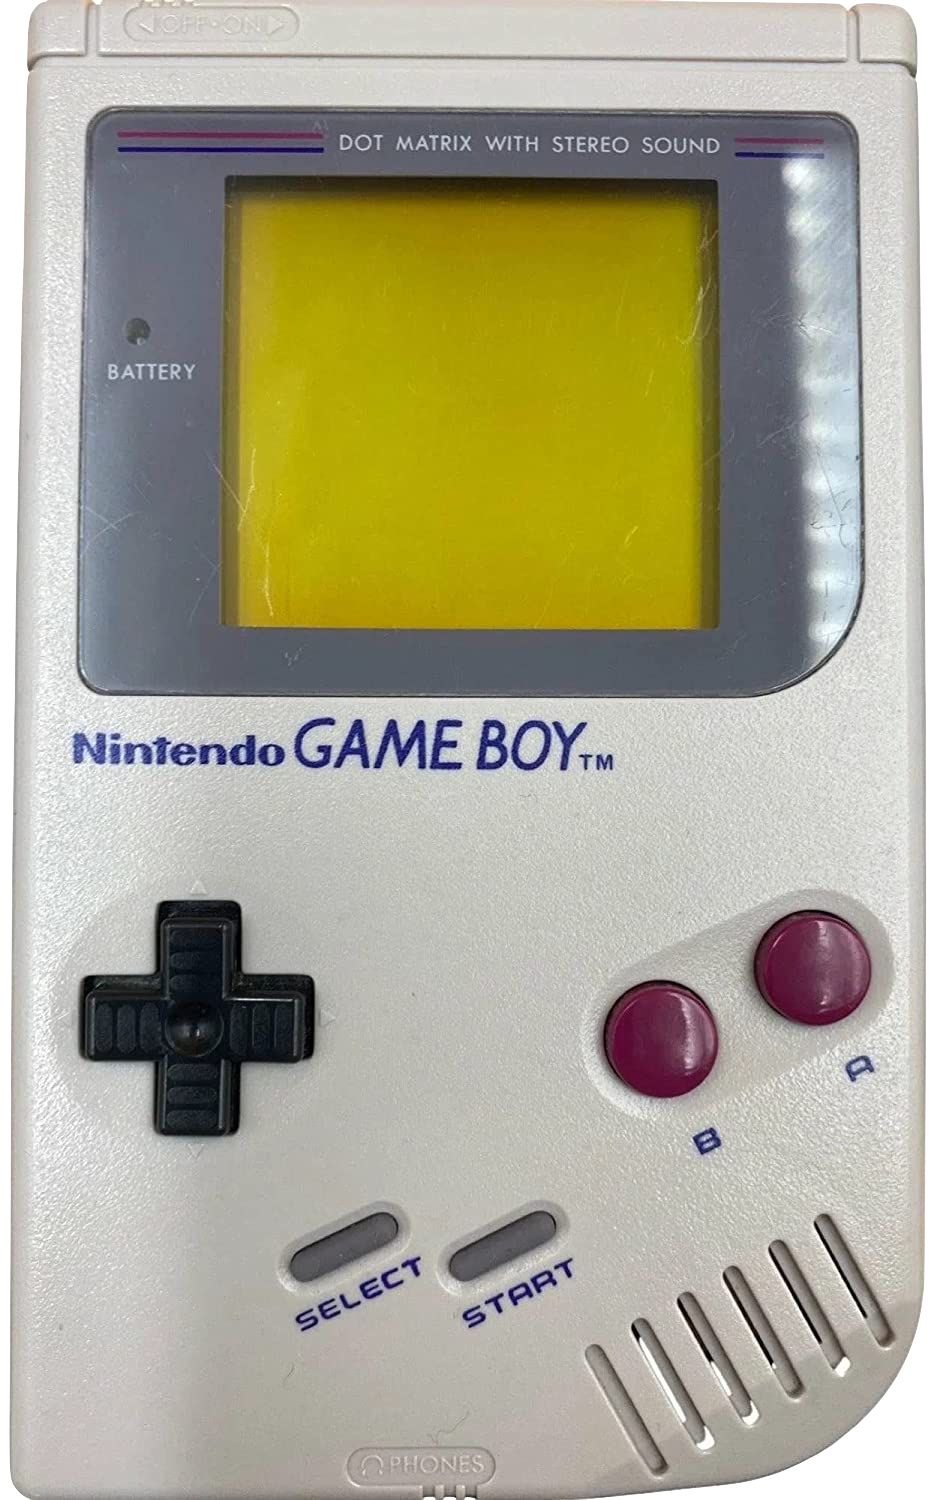
\includegraphics[width=4cm]{images/gameboy}\\
    \caption{Picture of a Gameboy, with the screen and joypad visible}
    \label{fig:gb-front}
\end{figure}

\section{System Bus}

Components withing the Gameboy need to communicate. To do this, components typically have a set of registers that control how they behave - for instance, the timer has a \texttt{TAC} register at \texttt{0xFF07} to control it's frequency. To allow this interaction without having all components directly depend on each other, a ``system bus'' component is created, responsible for handling all components and managing memory-addressing among them.

This component, called \texttt{System}, is thus responsible for instantiating the other components, and providing them access to eachother, via a read and write method.

\section{Other Components}

Aside from the aforementioned components, the \gls{gb} has a few components that allow it to run but aren't part of the \gls{cpu} or the input/output components. These will be briefly outlined here, as they have a lesser impact on the emulator's design.

\subsection{Timer}

The timer, responsible for incrementing a counter (the \texttt{DIV}) at a set frequency. It can raise interrupts, and owns a few registers.

\subsection{Interrupts}

The interrupt system, that allows components such as the timer or the \gls{ppu} to interrupt the \gls{cpu} to run another process. It can also be enabled and disabled by the \gls{cpu}, with the \texttt{EI} and \texttt{DI} instructions.

This sub-system is designed as a separate component to reduce coupling between other components, and instead have a small object that can be passed to components as needed.

\subsection{MBC}

The \glsfirst{mbc} is an extra chip contained within some game cartridges, to allow access to more \gls{rom} data (as well as external RAM in some cases) via banking \cite[MBCs]{pandoc}. There are multiple different \glspl{mbc}, and so it is convenient to define a common interface for all of them, which can then be implemented according to specification for each \gls{mbc} type.

The type of the \gls{mbc} is in the header of the \gls{rom} \cite[The Cartridge Header]{pandoc}. To separate this logic from the base system, a \texttt{ROM} class is used. It is responsible for reading the cartidge's header, and creating the appropriate \gls{mbc} instance.

\section{Useful Classes}

To have similar interfaces over all components, we will also declare specific classes and interfaces to be implemented by them.

\subsection{Addressable}

The \texttt{Addressable} interface provides a read and write method. This allows all components to communicate between each other without needing to be aware of what the component they're communicating with is. Aside from the \gls{cpu}, all components of the emulator implement this method.

\subsection{Memory and registers}

Simple utility classes can be declared to manage memory in a simple way.

The \texttt{RAM} class implements \texttt{Addressable}. It can be instantiated with a set size, and can be read and written to. It is used in components that have large blocks of writable data.

The \texttt{Register} class implements \texttt{Addressable}, but ignores the address parameter of the read and write operations, as it contains only one byte. A \texttt{DoubleRegister} class may also be implemented, backed by two \texttt{Register}s, to provide support for 16-bit registers, used for instance in the \gls{cpu}.

\chapter{Implementation}

The project uses Preact\ftnt{https://preactjs.com/}, a light-weight alternative to the more popular React\ftnt{https://reactjs.org/} framework. Preact was chosen because the front-end of the web-app is extremely lightweight, so a smaller framework with less features is enough. This also avoids bloating the app with a heavy framework such as React: its GZipped and minified size is around 31.8Kb, while Preact is only 4Kb (87\% less).

The language used for the project is TypeScript\ftnt{https://www.typescriptlang.org/}, a typed version of JavaScript. This is essential for the project, as ensuring the correctness of code can be extremely hard without proper typing constraints, especially as a project grows in size.

The project is divided into two parts:
\begin{compactitem}
    \item The \texttt{frontend/} directory contains the UI for the web-app. The main logic to create the emulator and run it is contained in \texttt{app.tsx}.
    \item  The \texttt{emulator/} directory contains the actual \gls{gb} emulator. Although most classes and interfaces used are exported, only three elements are needed to properly interact with the emulator:
    \begin{compactitem}
        \item \texttt{GameBoyColor.ts} handles the core loop of the system. It contains the \texttt{GameBoyColor} class, the emulator. Instantiating the emulator creates all the necessary sub-components, and calling the \texttt{drawFrame()} method runs the emulator for one frame (0.16 seconds).
        \item \texttt{GameBoyOutput.ts} contains a simple interface, with optional methods to receive any output produced by the emulator (see figure~\ref{fig:gameboyoutput}). The two main methods of this are \texttt{receiveGraphics} and \texttt{receiveSound}, which use the output of the actual console.
        \item \texttt{GameBoyInput.ts} contains a simple interface with a required \texttt{read()} method that returns an object with the current inputs for the console (see figure~\ref{fig:gameboyinput}).
    \end{compactitem}
\end{compactitem}

\begin{figure}[h]
    \begin{minted}{typescript}
interface GameBoyOutput {
    receiveGraphics?(data: Uint32Array): void;
    receiveSound?(data: Float32Array): void;

    // Debugging methods:
    debugBackground?(data: Uint32Array): void;
    debugTileset?(data: Uint32Array): void;
    serialOut?(data: number): void;
}
    \end{minted}
    \caption{\texttt{GameBoyOutput} interface methods}
    \label{fig:gameboyoutput}
\end{figure}

\begin{figure}[h]
    \begin{minted}{typescript}
type GameBoyInputRead = {
    up: boolean;
    down: boolean;
    left: boolean;
    right: boolean;

    a: boolean;
    b: boolean;
    start: boolean;
    select: boolean;
};

interface GameBoyInput {
    read(): GameBoyInputRead;
}
    \end{minted}
    \caption{\texttt{GameBoyInput} interface method}
    \label{fig:gameboyinput}
\end{figure}

\section{Emulator Frontend}

The frontend of the emulator is written in Preact, allowing us to create a simple, fast and lightweight UI to control it. It contains the emulator title, the control buttons and the emulator video output (see figure~\ref{fig:emmy-home}). Along the left of the screen is a sidebar with more options, allowing the user to customise the emulator to their needs and debug the state of the console if needed.

\begin{figure}[h]
    \centering
    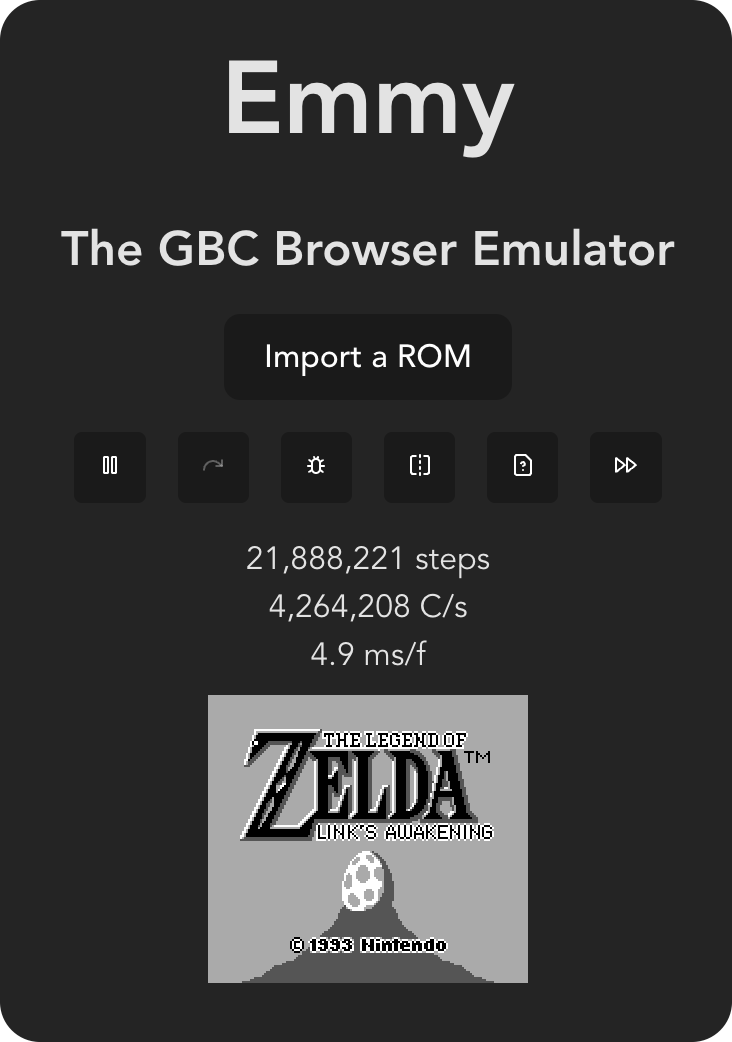
\includegraphics[width=15cm]{images/emmy-home-page}\\
    \caption{Home page of the emulator}
    \label{fig:emmy-home}
\end{figure}

\subsection{Main Controls}

The main controls for the emulator are the 6 buttons above the screen. These are, from left to right:

\begin{compactitem}
    \item Pause/play: pauses or resumes the emulator.
    \item Step by one \gls{cpu} instruction: this is a feature useful for debugging the emulator, when precise information of the state of the emulator is needed.
    \item Sound toggle: allows enabling or disabling the sound of the emulator. By default the sound is turned off, because modern browsers don't allow websites to play any sound before the user interacts with the website \cite{browser_autoplay}.
    \item Triple speed toggle: a toggle button that speeds up the emulator to emulate the \gls{gb} thrice as fast as usual. This is a common feature found in most emulators.
    \item Save state: saves the current state of the cartridge in the browser's storage, allowing the user to resume playing the game later. Note this doesn't save the full state of the emulator, but that of the cartridge, making it equivalent to a real-life save on the \gls{gb} where only the battery-backed storage of the cartridge persists through power-offs.
\end{compactitem}

\subsection{Settings}
\label{sec:settings-ui}

In the side drawer, the first tab is ``Settings''. It contains general settings for the emulator, such as:

\begin{compactitem}
	\item the console used by the emulator. This may either be the \gls{dmg} or the \gls{gbc}.
	\item an extra filter to be applied to the output. This increases the resolution of the screen, using the Scale2x or Scale4x\ftnt{https://www.scale2x.it/} algorithm (see \ref{fig:scale-filter}).
	\item the size of the emulator's screen, allowing resizing to two or four times larger.
	\item a slider to change the volume of the emulator's audio output.
	\item a palette selector, to change the four hues of the \gls{dmg}'s screen.
	\item two buttons to uploda the boot \glspl{rom} of the \gls{dmg} and \gls{gbc}. This is needed for users that wish to play with the full start-up screen of the console, as these two \glspl{rom} are copyrighted and cannot be distributed. If they're not provided, the emulator simulates their effect on the system.
	\item miscellaneous togglable settings, grouped together:
	\begin{compactitem}
		\item an option to play with or without the initial boot \gls{rom} of the emulator (a boot \gls{rom} must have been uploaded).
		\item a toggle to enable frame-blending, meaning for every new frame the output is mixed with the previous frame. This is a nice addition to have, because certain games made certain objects flicker on screen to make them appear translucent (since the flicker wasn't visible to the eye).
		\item a button to show the performance statistics of the emulator. This is mainly useful when developing the emulator to make sure it is still efficient.
		\item a toggle to enable the debug view of the emulator, where the currently loaded tileset and background map are displayed (see \ref{fig:debug-view}).
	\end{compactitem}
\end{compactitem}

\begin{figure}[h]
    \centering
    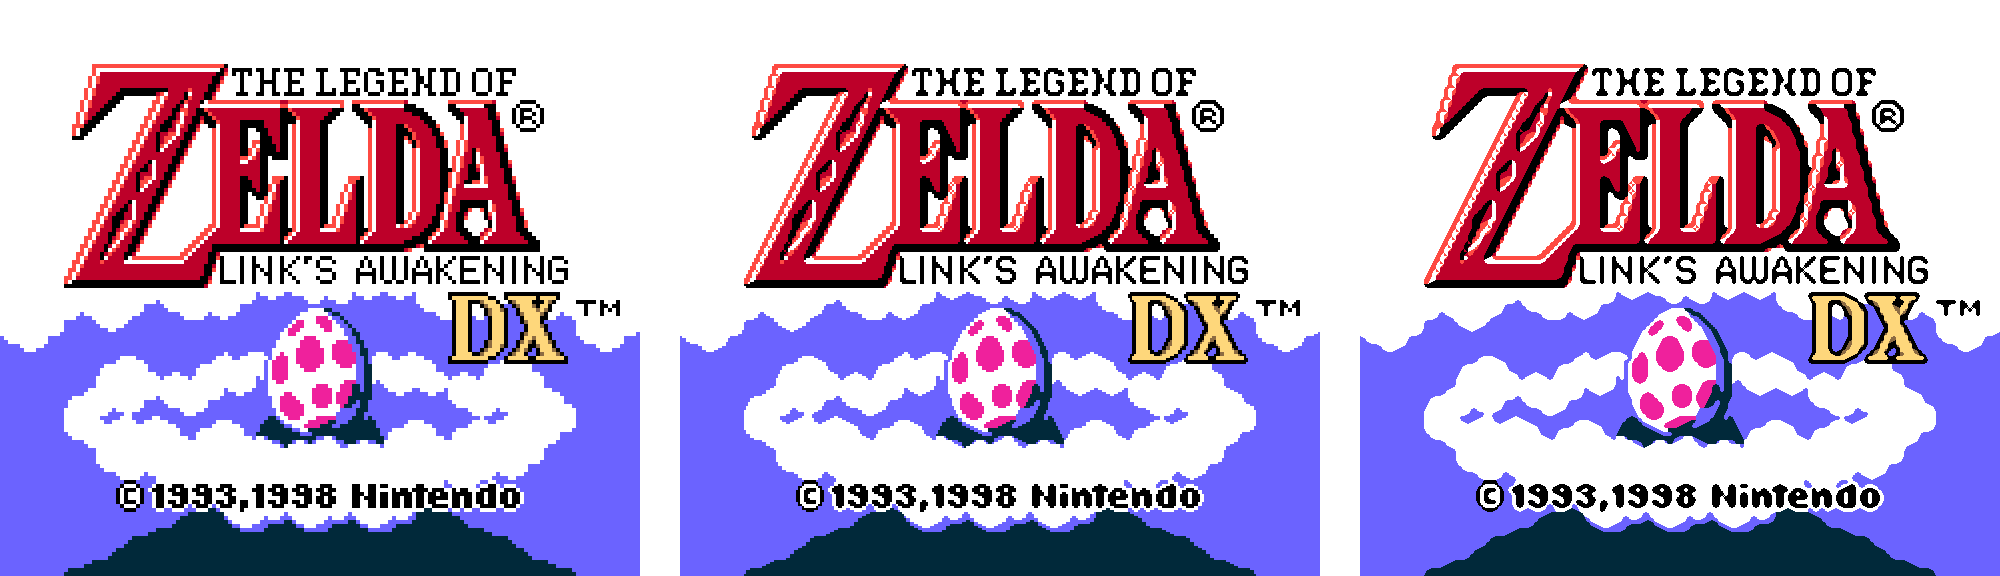
\includegraphics[width=15cm]{images/scale-filter}\\
    \caption{Output of the \gls{gbc} with, from left to right: no filter, Scale2x and Scale4x}
    \label{fig:scale-filter}
\end{figure}

\begin{figure}[h]
    \centering
    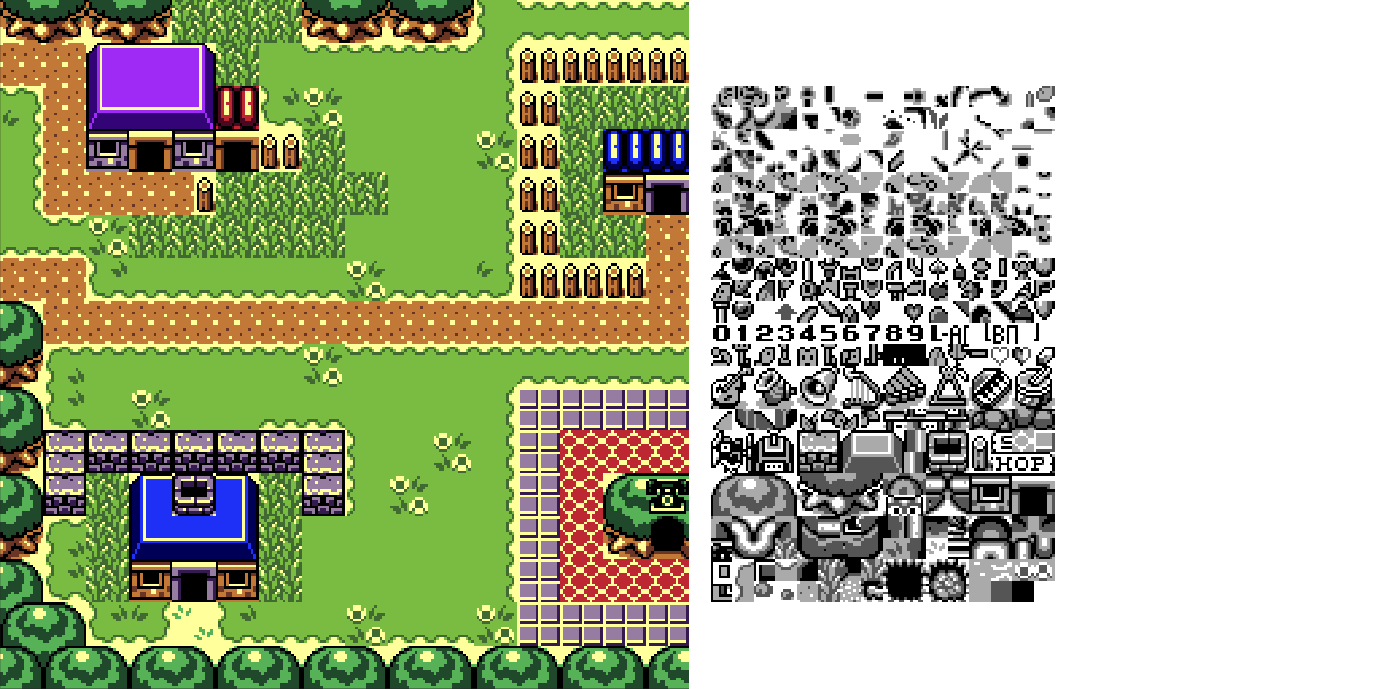
\includegraphics[width=10cm]{images/debug-view}\\
    \caption{Debug view of the emulator}
    \label{fig:debug-view}
\end{figure}

\subsection{Watch Expressions}

The second drawer allows the user to define custom JavaScript functions to inspect the state of the emulator regularly (see \ref{fig:watch-expressions}). This requires knowledge of the inner structure of the emulator, as the field names need to be used, but is quite useful when needing to inspect parts of the console that aren't the memory, like internal counters used for components, or register values.

To implement this, the \texttt{Function}\ftnt{https://developer.mozilla.org/en-US/docs/Web/JavaScript/Reference/Global_Objects/Function/Function} constructor is used, which takes in a string with the function's code. This allows the user to dynamically change the expression, and the component will simply update the function, without needing to reload the whole application. These expressions are also automatically saved to \texttt{localStorage}\ftnt{https://developer.mozilla.org/en-US/docs/Web/API/Window/localStorage}, meaning they will be kept between sessions.

The user-defined function is then repeatedly invoked, and the result output below the expression, allowing for a live-status of the emulator. If an error is thrown by the function (due to a null value, or invalid expression), the error is caught and `\texttt{Error}' is displayed.

\begin{figure}[h]
    \centering
    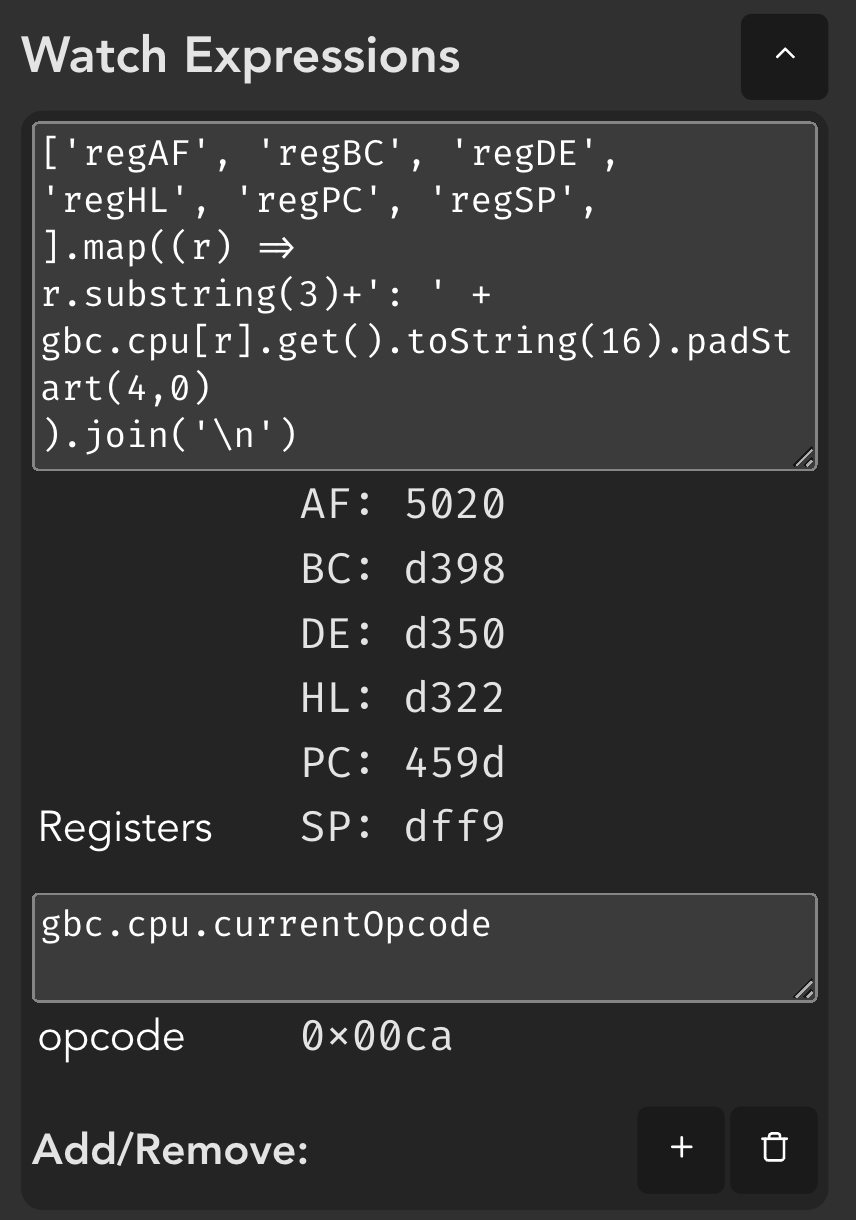
\includegraphics[width=5cm]{images/watch-expressions}\\
    \caption{Watch expressions drawer}
    \label{fig:watch-expressions}
\end{figure}

\subsection{Test ROMs}
\label{sec:testing-ui}

To ensure emulators work properly, a variety of test \glspl{rom} have been made, that test most aspects of the \gls{gb} (see \ref{sec:gb-test-roms}). The front-end of the emulator supports running a large number of them in an automated way (see \ref{fig:}). The user can select the group of tests desired by ticking the associated, or select/unselect everything by pressing the top right button. They can then run them by pressing the ``Test'' button, making them run internally (without receiving any input our outputting anything directly). The status of each individual test is displayed, and the user can click on the test name to run it on the main emulator, for further debugging or inspection.

\begin{figure}[h]
    \centering
    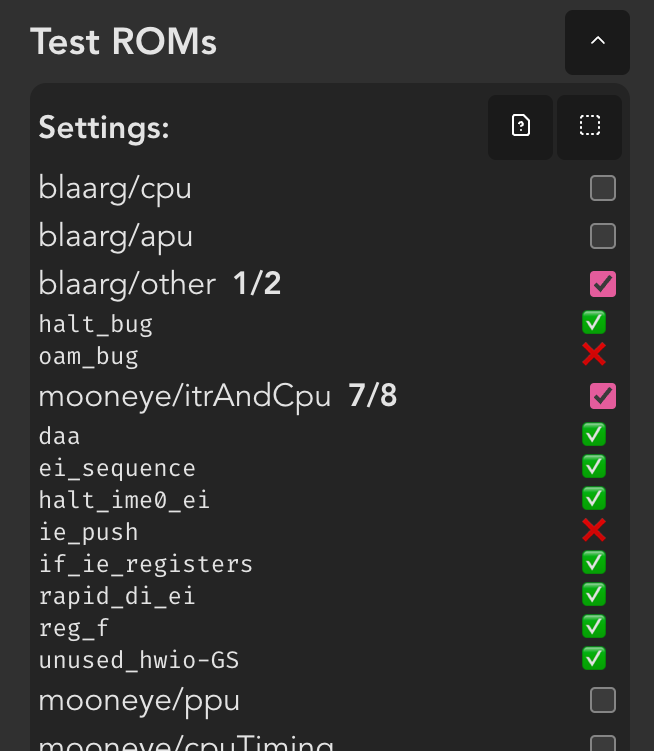
\includegraphics[width=5cm]{images/test-roms}\\
    \caption{Test \glspl{rom} drawer}
    \label{fig:watch-expressions}
\end{figure}

To run the tests, an emulator instance is created, with the test \gls{rom} as the input data and ``spy'' objects provided for input and output - these spies store the output of the emulator, to evaluate the state of the test. To stop execution, the emulator's state is inspected regularly, and the outcome of the test is checked (with execution terminating if the test takes too long to end).

To detect the outcome of each test, these are grouped according to what test suite they belong to. Each test suite is then associated to a \textit{success function}, that can either return \texttt{"success"}, \texttt{"failure"} or \texttt{null} if no outcome has been reached yet. As such, all tests in a test suite have a similar way of reporting success and failure.

The currently automated test suites are:
\begin{compactitem}
	\item The Blaarg test \glspl{rom}\ftnt{https://github.com/retrio/gb-test-roms}. The success function of this suite is quite complex, as this suite doesn't have a standard way of outputting the result. As such multiple parts of the emulator are inspected simultaneously:
		\begin{compactitem}
			\item \texttt{"Passed"}\footnote{See lines 50-54 of \texttt{mem\_timing/source/common/testing.s} in \url{https://github.com/retrio/gb-test-roms}} and \texttt{"Failed"}\footnote{See lines 112-139 of \texttt{mem\_timing/source/common/runtime.s} in \url{https://github.com/retrio/gb-test-roms}} may be output to the console's serial port.
			\item If the memory at \texttt{0xa001-0xa003} is equal to \texttt{0xdeb061}, then the byte stored at \texttt{0xa000} is the status of the test\footnote{See `Output to memory' in \texttt{dmg\_sound/readme.txt} of \url{https://github.com/retrio/gb-test-roms}}.
			\item For the \texttt{halt\_bug} test, there doesn't seem to be anywhere where the result is output, so the graphical output of the emulator is verified.
		\end{compactitem}
	\item The Mooneye test \glspl{rom}\ftnt{https://github.com/Gekkio/mooneye-test-suite} and SameSuite\ftnt{https://github.com/LIJI32/SameSuite/}, of which all tests are verified the same way. In case of success, the \texttt{B}, \texttt{C}, \texttt{D}, \texttt{E}, \texttt{H} and \texttt{L} registers hold the values $3$, $5$, $8$, $13$, $21$ and $34$ respectively (Fibonacci's sequence). If they instead all hold the value \texttt{0x42}, the test failed\footnote{See \url{https://github.com/Gekkio/mooneye-test-suite/\#passfail-reporting} for the Mooneye test suite, see lines 265-281 of \texttt{include/base.inc} in \url{https://github.com/LIJI32/SameSuite/} for the SameSuite}.
	\item The Acid test \glspl{rom} (\gls{dmg}\ftnt{https://github.com/mattcurrie/dmg-acid2}, \gls{gbc}\ftnt{https://github.com/mattcurrie/cgb-acid2}). These need to be tested graphically, as their purpose is verifying the actual output of the emulator rather than it's behaviour.
\end{compactitem}

Thanks to this, the emulator's frontend supports a total of 191 automated test \glspl{rom}, that verify the behaviour of most of the emulator. Of these 191 tests, 101 pass.

\subsection{Memory Inspect}

When debugging an emulator, being able to inspect it's memory is essential, as some bugs may be caused by the wrong mapping of components, or a fault when writing data. To help debugging this, the frontend comes with a basic memory inspection tool, that can show the entirety of the \textit{addressable} data of the emulator (see \ref{fig:memory-inspect}). This means data that is not accessible by the game (for instance, because the appropriate \gls{rom} bank is not selected) cannot be inspected here. A simple offset can also be indicated, to restrain the data to a certain area.

\begin{figure}[h]
    \centering
    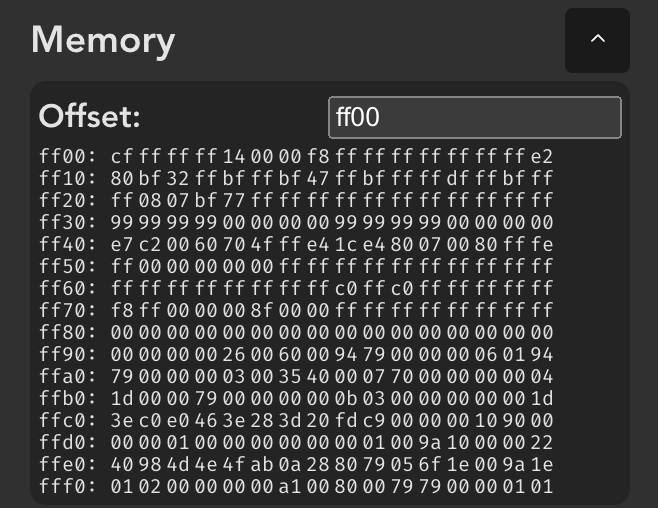
\includegraphics[width=5cm]{images/memory-inspect}\\
    \caption{The memory inspection drawer}
    \label{fig:memory-inspect}
\end{figure}

\subsection{Keybindings}

The user can also customise their keybindings for the emulator, by mapping each input to a separate key (see \ref{fig:keybindings}). This is only relevant on keyboard-equipped devices.

\begin{figure}[h]
    \centering
    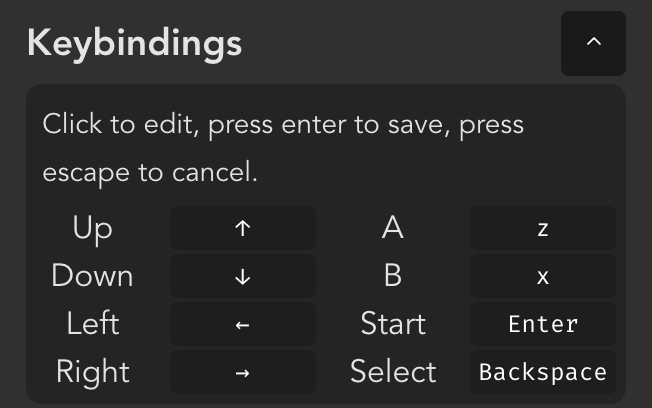
\includegraphics[width=5cm]{images/keybindings}\\
    \caption{The keybindings settings}
    \label{fig:keybindings}
\end{figure}

\section{Emulator-Frontend Interfaces}

To allow the emulator to communicate with the frontend, three components were created, each responsible for part of the output/input. 

\subsection{Screen output handler}

To allow easily displaying graphics data from the emulator on the frontend, a \texttt{Screen} component was created. This highly configurable screen takes multiple inputs, to allow configuring the screen's size, scale, if it has any upscaling filters applied, if it has any color palettes, and if it needs to blend frames together (see figure \ref{fig:screen-params}).

\begin{figure}[h]
    \begin{minted}{typescript}
type VideoReceiver = (data: Uint32Array) => void;
type ScreenProps = {
    inputRef: MutableRef<VideoReceiver | undefined>;
    width?: number;
    height?: number;
    scale?: number;
    Filter?: ImageFilter;
    blending?: boolean;
    id?: string;
    palette?: Partial<Record<number, number>>;
};
    \end{minted}
    \caption{Parameters of the \texttt{Screen} component}
    \label{fig:screen-params}
\end{figure}

All of the parameters are optional, and use sensible defaults when not specified. The only required parameter is \texttt{inputRef}, a modifiable ``pointer'' to the screen input function. This allows passing data to the screen without re-rendering the whole website. Because pointer's don't exist in TypeScript, what is passed is actually an object with a modifiable \texttt{value} field.

Whenever any parameter changes, a new \textit{render function} is generated, and is set in the given ``pointer''. This function takes as input the graphics data (a \texttt{Uint32Array}\ftnt{https://developer.mozilla.org/en-US/docs/Web/JavaScript/Reference/Global_Objects/Uint32Array}, containing ARGB values), and applies the required transformations to it. The function also holds a reference to two backing data buffers, for the previous and the current frame. This allows for blending between frames, and avoids creating new arrays repeatedly, lowering the memory consumption of the screen. The transformations it applies are: 

\begin{enumerate}[itemsep=0mm]
	\item Roll the buffers, setting the previous frame to the current frame, and the current frame to the newly received frame.
	\item If needed, apply the colour palette to the input. The palette is a simple map, from source colour to target colour.
	\item If it's the first frame to be drawn, also set the previous frame to the newly received frame (this avoid blending the new frame with a black frame, since the buffers are initialised with \texttt{0x000000} values).
	\item If required, blend the previous frame and the current frame.
	\item Apply the upscale filter to the image (this can be an identity filter, that simply returns the image, or upscale filters like Scale2x and Scale4x).
	\item The image data is created from the \texttt{Uint32Array}, and drawn on the \texttt{<canvas />}.
\end{enumerate}

This simple pipeline of functions makes the code really easy to understand and potentially modify, and allows for easy extension, as any filter could be given to the screen and it would work seamlessly. It is also of interest to note that the order in which the operations are applied maximised efficiency. For instance, the filter is applied last, to avoid having to do previous operations like blending on much larger images.

\subsection{Audio output handler}

To output the sound generated by the emulator, a utility class \texttt{AudioPlayer} was made. It is a simple class, that creates an \texttt{AudioContext}\ftnt{https://developer.mozilla.org/en-US/docs/Web/API/AudioContext} instance on creation. This class allows playing sound output from the browser.

A difficulty with playing audio data stems from the fact that audio samples are quite short (they are output every frame, so every $16.6$ milliseconds), and they must be constantly output, with tolerance for small delays in the output. If there happens to be even a small gap between two consecutive samples, a audible pop might play, which results in a very unpleasant experience.

To avoid this, \texttt{AudioPlayer} actually adds a small delay before starting to play audio. This ensures that by the time the first received sample is done playing, a new sample has already been received and queued for output, meaning there are never gaps between samples (except if there is an exceptionally long delay between samples, which shouldn't happen).

A drawback from this solution however is that if samples are received too fast, a delay may create itself, as too many samples are enqued, and new samples need to wait for all the previous ones to be played before being played. To avoid having this delay grow too large, a parameter of \texttt{AudioPlayer} allows setting the max size of the enqueued audio samples (the frontend uses a value of 8) - any samples that would make the queue exceed this size are ignored, meaning the max delay of the playback is $8*\frac{1}{60}=0.13$ seconds, a reasonable delay.

\subsection{Input handler}

To provide a simple way of handling inputs whether the device has a keyboard or uses touch controls, a \texttt{GameInput} component was created. It handles keyboard inputs, via a helper hook\ftnt{https://reactjs.org/docs/hooks-intro.html}, \texttt{useKeys}. To handle touch screen inputs, this component creates buttons mimicking those of the \gls{gb}. These buttons all have the \texttt{mobile-only} class, which is defined in \texttt{main.css} to only be visible when no fine pointer is available on the device (ie. no mouse is detected), as can be seen on figure \ref{fig:css-mobile-only}.

\begin{figure}[h]
    \begin{minted}{css}
@media (any-pointer: fine) {
    .mobile-only {
        display: none;
    }
}
    \end{minted}
    \caption{\texttt{mobile-only} CSS class}
    \label{fig:css-mobile-only}
\end{figure}

This means that if the user is on a mobile devices, the buttons will show, allowing for input without the need for a keyboard (see figure \ref{fig:ui-mobile-buttons}).

\begin{figure}[h]
    \centering
    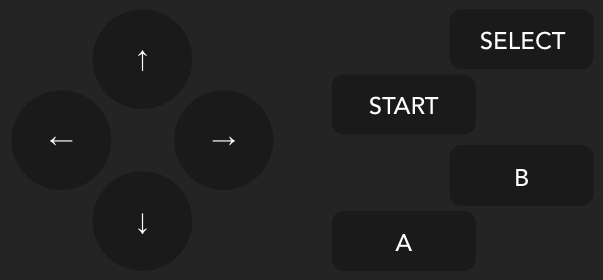
\includegraphics[width=5cm]{images/ui-mobile-buttons}\\
    \caption{Buttons for mobile devices}
    \label{fig:ui-mobile-buttons}
\end{figure}

The component itself then takes as a parameter a callback, that is called with the input function created by this component and returns an up to date object with the currently read inputs \texttt{GameBoyInputRead} (see figure \ref{fig:gameboyinput}).

\section{CPU}

The \gls{cpu} is the core of the emulator, and allows running the code from the \gls{rom} by reading the operation code (or opcode) and executing the matching action.

\subsection{Instruction Set Decoding}

Because the \glsdesc{gb} is an 8-bit system, opcodes are 8 bits (or one byte) long, giving in theory a maximum of $2^8=256$ operations. However in the \gls{gb} the operation \texttt{0xCB} gives access to an extended instruction set, meaning that when reading \texttt{0xCB} the \gls{cpu} will read the next byte and use a different logic to execute the operation. This means there are now $2^8 - 1 + 2^8=511$ operations. The \gls{gb} also has 11 `unused' opcodes, that will lock the console when used\cite[CPU Comparison with Z80]{pandoc}, meaning there are in total $2^8 - 12 + 2^8 = 500$ operations to implement.

Multiple techniques exist to handle this large number of operations:

\begin{compactitem}
    \item Have a large switch-statement for all possible operations. This is the most straight-forward option, but can result in quite large switch-statements, especialy for \glspl{cpu} with more opcodes. The \gls{gb} has comparatively few opcodes as it is an 8-bit system; the Gameboy Advance, the console that followed it, had 32-bit opcodes: way too many for a switch statement to be appropriate.
    \item Decode the operation by reading specific parts of the opcode, and generate the instructions dynamically. This method is what is done for larger instruction sets, where opcodes can be split into separate parts to describe the operation's behaviour \cite[ARM CPU Reference]{gbatek}. It however comes with the cost of extra processing for each instruction, as it needs to be decoded. This method is applicable to the \gls{gb}, as many instructions follow a pattern - see, for instance the \texttt{LD} instructions, that all follow the same order of registers: \texttt{B}, \texttt{C}, \texttt{D}, \texttt{E}, \texttt{H}, \texttt{L}, \texttt{(HL)} (the byte at address \texttt{HL}) and \texttt{A}.
    \item Create a dispatch table a map that associates each opcode to a function to execute \cite{dispatch_table}. This technique is also only viable for small numbers of opcodes, as the map can result quite large. An advantage of this method is that the map doesn't have to be explicitly written out entirely - generators can be used to populate some chunks of it, making it a hybrid of the two previous solutions: there is very little overhead to execute an instruction, as each opcode is associated to a function, but there is also no need to write out every instruction separately, as the map can be generated in parts or in its entirety (inducing a light setup cost).
\end{compactitem}

Initially, the emulator had a large map, with all the opcodes as keys. The functions associated would then execute the instruction and return the number of cycles taken by the instruction (see figure~\ref{fig:instset-first}). This however proved quite repetitive and prone to errors. To solve this, a \textit{generator function} was created. To use it, two parameters must be given: a map of opcodes to values (of an arbitrary type), and a helper function that for each arbitrary value returns a function that executes the instruction (see figure~\ref{fig:cpu-gen-function}). This allows generating repetitive instructions more easily, by only specifying what opcodes and objects are used, and not what the whole body of the instruction is (see figure~\ref{fig:instset-second}). This method is used in other emulators - for instance, Sameboy has a map that has an opcode-function mapping for all opcodes, and uses macros to generate the different functions\ftnt{https://github.com/LIJI32/SameBoy/blob/master/Core/sm83\_cpu.c}.

\begin{figure}[h]
    \begin{minted}{typescript}
protected instructionSet: Partial<Record<number, InstructionMethod>> = {
    // NOP
    0x00: () => 1,
    // LD BC/DE/HL/SP, d16
    0x01: (s) => { this.regBC.set(this.nextWord(s)); return 3; },
    0x11: (s) => { this.regDE.set(this.nextWord(s)); return 3; },
    0x21: (s) => { this.regHL.set(this.nextWord(s)); return 3; },
    0x31: (s) => { this.regSP.set(this.nextWord(s)); return 3; },
    ...
}
    \end{minted}
    \caption{Initial instruction set implementation}
    \label{fig:instset-first}
\end{figure}

\begin{figure}[h]
    \begin{minted}{typescript}
protected generateOperation<K extends number, T>(
    items: Record<K, T>,
    execute: (r: T) => InstructionMethod
): Record<K, InstructionMethod> {
    const obj: Record<K, InstructionMethod> = {};
    for (const [opcode, item] of Object.entries(items)) {
        obj[opcode] = execute(item);
    }
    return obj;
}
    \end{minted}
    \caption{Generator function used for the CPU}
    \label{fig:cpu-gen-function}
\end{figure}

\begin{figure}[h]
    \begin{minted}{typescript}
protected instructionSet: Partial<Record<number, InstructionObject>> = {
    // NOP
    0x00: () => 1,
    // LD BC/DE/HL/SP, d16
    ...generateOperation(
        {
            0x01: this.regBC,
            0x11: this.regDE,
            0x21: this.regHL,
            0x31: this.regSP,
        },
        (register) => (s) => {
            register.set(this.nextWord(s));
            return 3;
        }
    ),
    ...
}
    \end{minted}
    \caption{Improved instruction set implementation}
    \label{fig:instset-second}
\end{figure}

\subsection{A cycle accurate CPU}

The Gameboy is a memory-bound system, meaning that it is limited by it's memory accesses. The \gls{cpu} can only execute either one read or one write per \gls{mcyc} \cite[CPU core timing]{gbctr}. It also needs to retrieve the opcode for each instruction, which takes an additional cycle, meaning an instruction performing no memory accesses lasts one cycle, and an instruction performing $n$ memory accesses lasts at least $n + 1$ cycles. Finally, the \gls{gb} overlaps the last cycle of the execution with the fetching cycle for the next opcode - this will thus be of importance when implementing the fetching of the opcode. See figure \ref{fig:ld-instr-timing} for the breakdown of an instruction.

\begin{figure}[h]
	\centering
    \begin{tikztimingtable}[timing/wscale=0.8]
      M-cycle & X 8D{M1} 8D{M2} 8D{M3} 8D{M4/M1} X \\
      Instruction & ; [opacity=0.4] 9D{Previous} ; [opacity=1.0] 24D{LD rr, nn} ; [opacity=0.4] X \\
      Mem R/W  & X 8D{R: opcode} 8D{R: lsb(nn)} 8D{R: msb(nn)} ; [opacity=0.4] 8D{R: next op} X \\
      Mem addr & X 8D{PC} 8D{PC+1} 8D{PC+2} ; [opacity=0.4] 8D{PC+3} X \\
    \end{tikztimingtable}

    \caption{Timing of the \texttt{LD rr, nn} instruction}
    Taken from GBCTR \cite[Sharp SM83 instruction set]{gbctr}
    \label{fig:ld-instr-timing}
\end{figure}


The current implementation is not \gls{mcyc} accurate: the \gls{cpu} instruction is executed as one monolithic block, rather than in different smaller parts. This becomes crucial when the timer, \gls{oam} and \gls{ppu} are involved, as they run in parallel with the \gls{cpu}, so memory accesses to these components may return different values depending on the \gls{mcyc}.

In all emulators that were found when researching for this project, \gls{mcyc} accuracy is reached by making the emulator ``\gls{cpu}-driven''. What this means is that inside each instruction, between each cycle, the \gls{cpu} is responsible for ticking the rest of the system - the main loop is then only responsible for continuously running the \gls{cpu}, and nothing else. This approach is probably the simplest and most straightforward one, as it is quite simple to implement - all one needs to do is call the system tick method when relevant (see figure~\ref{fig:cpu-driven-ld}).

Some emulator where this method was found:
\begin{compactitem}
	\item In Mooneye GB, this can be seen by the usage of the \texttt{CPUContext.tick\_cycle()} method when appropriate\footnote{See \url{https://github.com/Gekkio/mooneye-gb/blob/master/core/src/cpu.rs}}.
	\item In accurateboy, the \texttt{Bus.tick()} method is called from within the instructions (or it is done implicitly by methods such as \texttt{Bus.read()})\footnote{See \url{https://github.com/Atem2069/accurateboy/blob/master/accurateboy/CPU.cpp}}.
	\item In Sameboy, the \gls{cpu} uses functions like \texttt{cycle\_read} or \texttt{cycle\_no\_access} to tick the rest of the system\footnote{See \url{https://github.com/LIJI32/SameBoy/blob/master/Core/sm83\_cpu.c}}.
\end{compactitem}


\begin{figure}[h]
    \begin{minted}{typescript}
protected ld_bc_hl(system: System) { // LD BC, (HL)
    const lower = system.read(this.regPC.inc());
    system.tick();
    const upper = system.read(this.regPC.inc());
    system.tick();
    this.regBC.set(upper << 8 | lower);
}
    \end{minted}
    \caption{CPU-driven \texttt{LD BC, (HL)}}
    \label{fig:cpu-driven-ld}
\end{figure}

This solution however comes with the cost of coupling the \gls{cpu} to the system, or at least to a way of ticking said system. A particularity of this emulator is that the \gls{cpu} is almost autonomous, in that it doesn't interact with any other functionality of the system, except the interrupts. The only other interface it requires being an \texttt{Addressable}, to allow access to memory. This also means the emulator is no longer ``\gls{cpu}-driven'', since the \gls{cpu} \textit{cannot} tick the rest of the system. It is instead up to the root system to tick all of the components (including the \gls{cpu}). This is thus a code quality improvement, that isn't present in other emulators.

This was done by splitting all the instructions into their respective steps, and have each step return the next step (or \texttt{null} if it's the last step). The \gls{cpu} now must simply store whatever the instruction returns: if it's \texttt{null} then it needs to fetch an instruction to prepare for the next cycle, otherwise it's a function and must be executed (and it's result stored for the next step). See figures \ref{fig:system-driven-ld} and \ref{fig:system-driven-cpu-tick} for an example of this.

In the final version of the \gls{cpu}'s tick method, a method \texttt{loadNextOp} is implemented. It not only handles getting an instruction associated with the desired opcode, but it also is responsible for checking if an interrupt was raised (in which case the interrupt handling procedure occurs \cite[Interrupts]{pandoc}), and for ensuring the \gls{cpu} isn't halted before running an instruction.

\begin{figure}[h]
    \begin{minted}{typescript}
protected ld_bc_hl(system: Addressable) { // LD BC, d16
    const lower = system.read(this.regPC.inc());
    return () => {
        const upper = system.read(this.regPC.inc());
        return () => {
            this.regBC.set(upper << 8 | lower);
            return null;
        }
    }
}
    \end{minted}
    \caption{System-driven \texttt{LD BC, d16}}
    \label{fig:system-driven-ld}
\end{figure}

\begin{figure}[h]
    \begin{minted}{typescript}
step(system: Addressable, interrupts: Interrupts) {
    if (this.nextStep === null) {
        // looks up opcode in instruction table
        const nextStep = this.loadNextOp(system, interrupts, verbose);
        if (nextStep === "halted") return true;
        this.nextStep = nextStep;
    }
    this.nextStep = this.nextStep(system, interrupts);
    if (this.nextStep === null) {
        // opcode is fetched on the last cycle of execution
        this.currentOpcode = system.read(this.regPC.inc());
    }
}
    \end{minted}
    \caption{System-driven step of the \gls{cpu}. Note how the opcode is fetched directly when the next instruction is over, to emulate the overlap between the fetch and the execute steps.}
    \label{fig:system-driven-cpu-tick}
\end{figure}


\section{System}

The \texttt{System} class implements the system bus, as well as the ticking of all other components. It handles the ticking of the \gls{ppu}, timer, \gls{apu} and interrupt logic. Furthermore, it is the component that links all of the data together: whenever a component is ticked (any of the above or the \gls{cpu}), the \texttt{System} instance is passed, so that the components can read and write to the rest of the system. It implements \texttt{Addressable} (see \ref{fig:addressable}), and internally has a \texttt{getAdress} method that returns the \texttt{Addressable} at this specific address, to be accessed in the \texttt{read} and \texttt{write} methods. This ensures that the logic used to determine what component is accessed depending on the address isn't duplicated.

\subsection{\texttt{getAddress} optimisation}

Because \texttt{System} is a higly used component and is accessed for almost every read and write, the \texttt{getAddress} method is under a lot of pressure: for a game like `The Legend of Zelda: Link's Awakening DX', the method is called around 650,000 times per second. For a more complex and resource-intensive game such as `Alone in the Dark: The New Nightmare', around 1,900,000 calls are made. This intensity in usage can easily be explained, as the \gls{gb} is a memory-bound system: almost all interactions between components occur through memory reads and write. \texttt{getAddress} must thus be optimised as much as possible, as it is one of the main bottle-necks of the emulator.

An initial implementation of \texttt{getAddress} used the combination of a list of if-statements for different ranges of the \gls{mmap}, as well as a map where all register addresses where mapped to the component responsible for them. The code would first check if the key exists in this map,,and if not it would then go through a series of if-conditions  (see figure~\ref{fig:getaddress-before}). It would not return a tuple, containing both \texttt{Addressable} to use and the address within in - this was needed as some components had a particular mapping to memory. This is the case for the \gls{wram}, who's memory starts at \texttt{0xC000} and ends at \texttt{0xFDFF} (spanning over 15.5KB bytes) despite it only being 8KB long, because the last 7.5KB of its address range map back to the beginning of it (this is called the Echo RAM \cite{memorymap}).

\begin{figure}[h]
    \begin{minted}{typescript}
protected getAddress(pos: number): AddressData {
    const register = {
        0xff00: this.joypad,
        ...
        0xffff: this.intEnable,
    }[pos];
    if (register !== undefined) return [register, pos];

    if (0x0000 <= pos && pos <= 0x7fff) return [this.rom, pos]; // ROM Bank
    ...
    if (0xfe00 <= pos && pos <= 0xfe9f) return [this.oam, pos]; // OAM

    // Unmapped area, return 'fake' register
    return [{ read: () => 0xff, write: () => {} }, 0];
}
    \end{minted}
    \caption{Initial implementation of \texttt{getAddress}}
    \label{fig:getaddress-before}
\end{figure}

This proved quite costly:
\begin{compactitem}
    \item This code creates a new map every time it is called, when checking for the registers' addresses.
    \item Having to return both an \texttt{Addressable} and an address is quite costly, as a new array with two items must be created every time. It also adds unecessary complexity to the method, as the system bus shouldn't be responsible for handling the details of address mapping, and instead simply delegate the task to the appropriate component.
    \item The if-conditions for the ranges of the biggest areas of memory (everything between \texttt{0x0000} and \texttt{0xEFFF}) happened after the register checks, which delayed response for these reads and writes. This is all the more important that this range represents $\frac{\texttt{0xEFFF}}{\texttt{0xFFFF}+1} \approx 93\%$ of the total address space.
    \item Chaining if-conditions is unneficient, as the JS engine must step through all conditions and check the values each time. Furthermore, although having both the lower and upper bound of the memory section indicated in the condition (e.g. \texttt{0x0000 <= pos \&\& pos <= 0x7FFF} for $[\texttt{0x0000}; \texttt{0x7FFF}]$) makes the translation from \gls{mmap} to code easier, it is slower, since only the upper bound of the range is needed for the condition if all the ranges below have already returned.
\end{compactitem}

First, we may move the fine-grained addressing logic to sub-components like the \gls{wram}. This removes the need to return an address from the method: only an \texttt{Addressable} is enough, as that component will then be responsible for decoding the address further.

The last two points may then be addressed, by removing the use of if-conditions, and moving this part of the code to the beginning of the function.

With the memory map of the console (see figure~\ref{fig:memory-map-largest}) we can notice how the largest chunks of memory all end with the last three nibbles of the address as \texttt{0xFFF}. This means that the component mapped to an address can be determined by simply looking at the first nibble of said address. This is probably done to simplify the circuitry responsible for addressing, as only the most significant 4 bits need to be compared. The emulator can take advantage of this.

\begin{figure}[h]
    \centering
    \begin{tabular}{|l|l|l|}
    \hline
    \textbf{Start} & \textbf{End} & \textbf{Description} \\ \hline
    \texttt{0000} & \texttt{3FFF} & 16 KB ROM bank 00 \\ \hline
    \texttt{4000} & \texttt{7FFF} & 16 KB ROM Bank 01$\sim$NN \\ \hline
    \texttt{8000} & \texttt{9FFF} & 8 KB Video RAM (VRAM) \\ \hline
    \texttt{A000} & \texttt{BFFF} & 8 KB External RAM \\ \hline
    \texttt{C000} & \texttt{CFFF} & 4 KB Work RAM (WRAM) \\ \hline
    \texttt{D000} & \texttt{DFFF} & 4 KB Work RAM (WRAM) \\ \hline
    \texttt{E000} & \texttt{FDFF} & Mirror of \texttt{0xC000}$\sim$\texttt{0xDDFF} \\ \hline
    \end{tabular}
    \caption{Memory map for the largest chunks of memory \cite{memorymap}}
\end{figure}

For this area of memory (\texttt{0x000}-\texttt{0xEFFF}) the system bus may simply isolate the most significant nibble, and then use a map to associate each address block to a component. Only if the address corresponds to \texttt{0xF-{}-{}-} do we try matching it to a register address. This removes the need for the if-conditions, and is also faster as it is evaluated much earlier on (see figure~\ref{fig:getaddress-after}). The map can be created on instantiation and kept for later use, to avoid unnecessary memory allocations.

\begin{figure}[h]
    \begin{minted}{typescript}
protected getAddress(pos: number): Addressable {
    // Checking last nibble
    let addressable = this.addressesLastNibble[pos >> 12];
    if (addressable) return addressable;

    // Registers
    if((address & 0xff00) === 0xff00) {
        addressable = this.addressesRegisters[pos & 0xff];
        if (addressable) return addressable;
    }

    if (pos <= 0xfdff) return this.wram;  // Echo RAM
    if (pos <= 0xfe9f) return this.ppu;   // OAM
    if (pos <= 0xfeff) return Register00; // Illegal Area

    return RegisterFF; // fake register
}
    \end{minted}
    \caption{Optimised implementation of \texttt{getAddress}}
    \label{fig:getaddress-after}
\end{figure}

To ensure placing the ``main block'' first was the best choice, measurements have been taken of four different \gls{gb} games. The emulator would log all memory accesses by groups of $100\,000\,000=10^8$, and categorise them by address ``blocks'': the main block, the \gls{oam} block, the illegal block (called like this because this area of memory is restricted by Nintendo, and only returns \texttt{0x00}) and the register block. This separation is justified by the fact these are the five chunks of memory that must be checked separately, due to their irregular boundaries. The \textit{second} set of $10^8$ accesses was then used to gather the statistics of what blocks are used the most. The first $10^8$ accesses aren't used, as they may include setup operations that only happen when the game loads, and as such don't represent what the average execution will look like. see figure~\ref{fig:access-rates} for the results.

% Data of the table:
% Alone in the Dark: { "most": 88_868_727, "echo": 0, "oam": 00_001_431, "illegal": 00_000_517, "registers": 11_129_325 }
% Link's Awakening DX: { "most": 95679115, "echo": 0, "oam": 0, "illegal": 0, "registers": 4320885 }
% Tetris: { "most": 84289047, "echo": 0, "oam": 0, "illegal": 0, "registers": 15710953 }
% Pokemon Silver: { "most": 95739934, "echo": 0, "oam": 0, "illegal": 0, "registers": 4260066 }

\begin{figure}[h]
    \centering
    \begin{tabular}{|l|l|l|l|l|l|}
    \hline
    \textbf{Name} & \textbf{Memory Area} & \textbf{Game 1} & \textbf{Game 2} & \textbf{Game 3} & \textbf{Game 4}  \\ \hline
    Main Block & \texttt{0x0000}-\texttt{0xEFFF}
    & 88.869\%
    & 95.679\%
    & 84.289\%
    & 95.740\% \\ \hline

    Echo RAM & \texttt{0xF000}-\texttt{0xFDFF}
    & 0.000\%
    & 0.000\%
    & 0.000\%
    & 0.000\% \\ \hline

    OAM Block & \texttt{0xFE00}-\texttt{0xFE9F}
    & 0.001\%
    & 0.000\%
    & 0.000\%
    & 0.000\% \\ \hline

    Illegal Block & \texttt{0xFEA0}-\texttt{0xFEFF}
    & 0.001\%
    & 0.000\%
    & 0.000\%
    & 0.000\% \\ \hline

    Register Block & \texttt{0xFF00}-\texttt{0xFFFF}
    & 11.129\%
    & 4.321\%
    & 15.711\%
    & 4.260\% \\ \hline
    \end{tabular}
    \caption{Access rate per memory blocks, for the second set of 10,000,000 accesses of 4 different games.}
    Games are, respectively, ``Alone in the Dark: The New Nightmare'', ``The Legend of Zelda: Link's Awakening DX'', ``Tetris'' and ``Pokémon Silver''.
    \label{fig:access-rates}
\end{figure}

As we can see, the great majority of memory accesses go to the main part of memory, with almost all of the rest going to the ``register area'', the last 256 bytes of the address space. This can easily be explained by the fact all registers that allow interaction with other components (the \gls{ppu}, the \gls{apu}, the timer, etc.) are in this narrow range, so it is bound to have a high usage. It is also quite interesting to note that neither the Echo RAM or the OAM block are used at all, except very rarely for one of the tested games. It is thus safe to assume that the conditions responsible for mapping these areas can be left at the end of the function, as they will rarely match an address.

\subsection{Evaluating the \texttt{getAddress} optimisation}

A simple experiment was then run, to verify the performance improvement. The first 25 million instructions of the \texttt{cpu\_instrs}\ftnt{https://github.com/retrio/gb-test-roms/tree/master/cpu_instrs} test \gls{rom} were run. This sample was chosen because it is considerably large, because the test itself requires around 25 million instructions to complete. For the measurement, \texttt{window.performance.now()}\ftnt{https://developer.mozilla.org/en-US/docs/Web/API/Performance/now} was used before and after each drawn frame, and the values were then summed.

The result was the following: $33\,955.9$ms before the change, and $20\,039.1$ after the change. The relative difference is thus $\frac{20\,039.1-33\,955.9}{33\,955.9}=-0.4098$, thus reducing time taken by $40.98\%$. By measuring the time spent within \texttt{getAddress} for these 25 million instructions, we get a total spent time in the method of $0.000\,151$ms on average, showing that this method is no longer a bottleneck for the system, as its impact on performance is minimal.

\section{PPU}

The \glsfirst{ppu} is the component responsible for rendering the game onto the Gameboy's screen. It is one of the most complex components of the \gls{gb}, with intricate timings, and a behaviour that changes between the \gls{dmg} and the \gls{gbc}, due to the addition of colour-support, as well as \glsfirst{vram} banking.

\subsection{Presentation}

The screen rendering is divided intro three layers, drawn on top of each other. From bottom to top, these are:

\begin{compactitem}
	\item The background, a $256 \times 256$ image loaded into memory that support scrolling on both axis.
	\item The window, similar to the background, is a $256 \times 256$ image that can be moved around the screen, and is toggleable. It however doesn't support scrolling.
	\item The objects, that are drawn at the very top, are smaller $8 \times 8$ tiles. These can be moved freely, and support some transformations, such as horizontal or vertical flipping. Their data is stored in the \glsfirst{oam}.
\end{compactitem}

It renders onto the screen line by line, meaning it will draw a 1-pixel wide line (the scanline) from left to right, and then proceed to the line below. Drawing an entire line takes 114 M-cycles, and there is an 1140 M-cycle delay when the bottom of the screen is reached. The advantage of having per-line rendering is that by modifying the position of the background between each drawn line, complex visual effects can be obtained quite easily \cite{gameboy_talk}, see figure~\ref{fig:background-transform} for an example.

\begin{figure}[h]
    \centering
    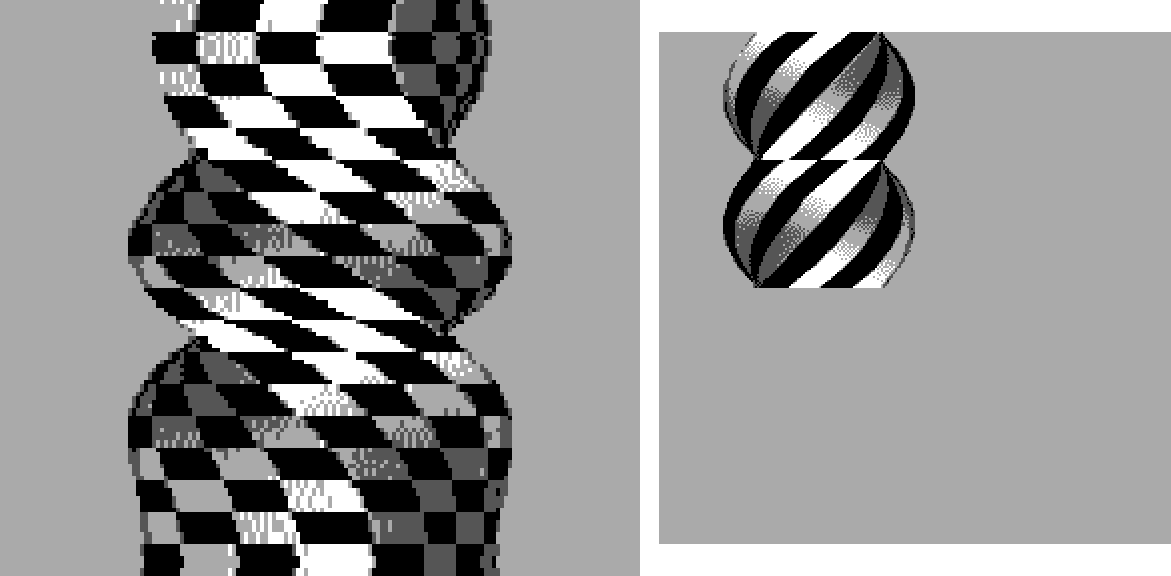
\includegraphics[width=8cm]{images/background-transform}\\
    \caption{Visual effects made by scrolling the background}
    Gameboy output (right), and loaded background data (right)
    \label{fig:background-transform}
\end{figure}

One of the main characteristics of the \gls{ppu} is that it operates in modes. During each mode, it perform a different set of operations, and can only be interacted with in certain way \cite[LCD Status Registers]{pandoc}. These four modes are:

\begin{compactitem}
	\item Mode 2: the \gls{ppu} looks through the \gls{oam}, to look for all the sprites to draw. During this time, the \gls{oam} is not accessible.
	\item Mode 3: the \gls{ppu} reads both the \gls{vram} and \gls{oam}, and draws the line. None of the video data is accessible here.
	\item Mode 0: the \gls{ppu} does nothing for a short length of time after each line. An interrupt is raised at the start of this period, allowing the \gls{cpu} to be notified now is the time to update what's rendered if necessary. This is called the horizontal blank, or HBlank.
	\item Mode 1: the \gls{ppu} does nothing for a long length of time after the bottom of the screen is loaded. This is usually where the bulk of the graphics update go, as it lasts a considerable amount of time (1140 \glspl{mcyc}). An interrupt is also raised here, to notify the \gls{cpu}. This is called the vertical blank, or VBlank.
\end{compactitem}

Rendering of the line is thus done during mode 3, when no graphics data is accessible, using a FIFO queue (First In First Out) of pixels that can be pushed in and out as the data is read. Some of the registers are still writable, but most games don't use them during this mode because they would require very precise timing. An example of a game relying on this is ``Prehistorik Man'', that changes the colour palette registers during the scanline in its intro-scene \cite[Tricky-to-emulate games]{gbdev_wiki}.

Since this is only the case for a minority of games, we can go past this inaccuracy. We'll thus take advantage of this to simplify greatly the rendering logic and make the renderer ``scanline based'', drawing an entire line all at once. This shortcut is commonly used by emulators that aren't too accuracy-oriented.

To handle each mode separately, we have four distinct ``mode'' objects of type \texttt{PPUMode}, that hold some basic information on the operation of the mode: it's length, it's flag for the \texttt{STAT} register and the name of the method in \texttt{PPU} responsible for ticking said mode (see figure~\ref{fig:stat-mode-type}). Note \texttt{KeyForType<T, V>} is the union of all keys \texttt{k} of \texttt{T} such that \texttt{T[k]} is of type \texttt{V}.


\begin{figure}[h]
    \begin{minted}{typescript}
type PPUMode = {
    doTick: KeyForType<PPU, (interrupts: Interrupts) => void>;
    flag: number;
    cycles: number;
};
    \end{minted}
    \caption{Type definition of \texttt{PPUMode}}
    \label{fig:stat-mode-type}
\end{figure}

\subsection{Rendering Logic}

The first step needed to render the game is to select and order all the sprites to be shown on screen. One of the limitations of the \gls{gb} is that despite having enough space in memory for 40 sprites, only 10 may be rendered at a time in a scanline \cite[OAM]{pandoc}. The sprites are selected during mode 2 - as such, during the last cycle of mode 2, the emulator will look through the available sprites in the \gls{oam}, and select the appropriate ones. This can be done quite elegantly in a functional manner, using an array (see figure~\ref{fig:sprite-select}).

\begin{figure}[h]
    \begin{minted}{typescript}
this.readSprites = this.oam
    .getSprites()
    .filter((sprite) => sprite.y <= y && y < sprite.y + objHeight)
    .slice(0, 10)
    .map((sprite, index) => [sprite, index])
    .sort(objPrioritySort)
    .map(([sprite]) => sprite);
    \end{minted}
    \caption{Retrieve the selected sprites for the scanline}
    \label{fig:sprite-select}
\end{figure}

First, we retrieve the sprites from the \gls{oam}. Internally, sprite data is cached between scanlines and invalidated when written to - \texttt{getSprites()} updates the dirty tiles in the cache and returns them. This avoid decoding the sprite every line if it doesn't receive changes, while also ensuring excess decoding isn't done if the sprite is modified twice between scanlines. We then select the first 10 sprites to be part of the scanline - this selection is done based on index: the \gls{ppu} looks through the \gls{oam} sequentially to find matching sprites \cite[OAM]{pandoc}. Finally, a re-ordering of the sprites needs to be done, to determine which sprite goes above which - this may depend on the sprite's position in the \gls{oam}, or on it's X coordinate. This is handled in \texttt{objPrioritySort}. To allow sorting based on both attributes, the sprites must be briefly remapped to a tuple with the sprite and it's index (as JavaScript doesn't expose the indices of elements when ordering them). These sprites are then stored in the \gls{ppu} object, to be used when rendering at the end of mode 3.

The \gls{ppu} uses a form of indirect addressing to handle data. It has an area in \gls{vram} that stores image data (tiles), $8 \times 8$ images. Whenever one of these tiles needs to be used, for the background, or for an object, the identifier of the tile needs to be used - this identifier being derived from the tile's address. This allows for the very simple re-use of tiles, which is particularly relevant for backgrounds where they may be repeated a lot. This background data is stored in a \textit{tile map}, a $256 \times 256$ map of 1-byte indices to the actual tile data. The \gls{gb} has two such maps, and both the background and window can display either of them - this is controlled via a flag in the \texttt{LCDC} register.

To render the scanline, the layers need to be drawn on top of each other: background, then window, then objects. Due to the similarities between background and window, a \texttt{drawLayer} method can be shared to handle the bulk of the work.

This method will loop over all tiles it needs to draw in the current scanline. It first needs to determine the tile's index. This index can be used to the retrieve the tile's address in \gls{vram}. It can also be used to fetch the attributes of the tile; this is a \gls{gbc}-exclusive feature, that allows transforming tiles (for instance, flipping them, or selecting a different palette for the tile). These attributes are stored in the second bank of \gls{vram}, at the same address, in a single byte of data. The \gls{dmg}/\gls{gbc} distinction isn't needed however, because the attributes for a \texttt{0x00} value match the attributes used by the \gls{dmg}. This means that instead of having two different branches to split the console versions, we can setup the \gls{dmg} emulator to always return \texttt{0x00} for the second bank of \gls{vram}, and keep the \gls{gbc} handling of attributes.

Once the tile index has been acquired, the \gls{ppu} may retrieve the tile data address from \gls{vram}. This one-byte address needs to be converted to a valid address in the tile data range of \gls{vram}, as it contains two partially overlapping tile data areas - a flag in the \texttt{LCDC} register controls this. Once the address where the tile data (ie. it's texture) is obtained, the \gls{ppu} may finally retrieve said data, and draw it in the scanline.

\begin{figure}[h]
    \centering
    \includegraphics{diagrams/ppu-logic.drawio.pdf}
    \caption{PPU logic to obtain tile data}
	This applies to the DMG - the CGB has two VRAM banks, thus having twice as many tile textures, and an additional tile attribute map.
    \label{fig:emu-core-components}
\end{figure}

This tile data, an $8 \times 8$ images where each pixel can be one of four shades is encoded in 16 bytes. Because tile data is rarely changed and the procedure to extract the image data from these 16 bytes is quite complex and requires some bit manipulation, tiles are cached.


\subsection{Subcomponents}

Although it is present to the system as a unit, the \gls{ppu} is implemented as multiple smaller-components, that handle different parts of the screen logic. This is all the more important that the \gls{ppu} is extremely complex, so care is needed to ensure the code remains maintainable.

The \glsfirst{oam} is the memory area in the \gls{ppu} that stores object data. This small 160-byte long area has a feature called \gls{oam} \glsfirst{dma}, allowing for direct transfers from ROM or RAM to the \gls{oam}. Because this transfer runs in parallel to the other components, the \gls{oam} itself is its own component, contained inside the \gls{ppu}. This allows for a better separation of concerns between the two - the \gls{ppu} handles rendering, the \gls{oam} handles OAM DMA and sprite storing and decoding.

The colour management of the \gls{ppu} also requires some extra logic that can be extracted into its own class. Although on the \gls{dmg} this is limited to splitting a byte into 4 shades of 2 bits (white, light gray, dark gray and black), the \gls{gbc} has a 16 palettes of 4 colours, 8 palettes for the background and window, and 8 for sprites \cite[Palettes]{pandoc}. As such, a \texttt{ColorController} class was created - it implements \texttt{Addressable}, and has a method to retrieve the palette for the background, and a method to retrieve the palette of a sprite. This class is extended by a \texttt{DMGColorController}, and a \texttt{CGBColorController}. The \texttt{PPU} picks one of the two on instantiation, based on the emulated console, and can then use both, without needing to know if the screen is monochrome or coloured.

Similarly, the \gls{vram} behaves slightly different between the \gls{dmg} and the \gls{gbc}: the latter's \gls{vram} has two banks it can switch between, via an additional register, and also supports \gls{vram} \gls{dma} transfers, similar to what is possible with the \gls{oam}. A \texttt{VRAMController} class is created - it also implements \texttt{Addressable}, and has a few extra methods, to allow getting tiles from it, and reading each bank individually (see figure~\ref{fig:vramcontroller-interface}).

\begin{figure}[h]
    \begin{minted}{typescript}
abstract class VRAMController implements Addressable {
    read(pos: number): number;
    write(address: number, value: number): void;

    tick(system: Addressable, isInHblank: boolean, isLcdOn: boolean): boolean;

    getTile(tileAddress: number, bankId: 0 | 1): Int2[][];
    readBank0(pos: number): number;
    readBank1(pos: number): number;
}
    \end{minted}
    \caption{Interface of \texttt{VRAMController}}
    \label{fig:vramcontroller-interface}
\end{figure}


\section{APU}

The \glsfirst{apu} is the component responsible for producing the sounds and music of the \gls{gb}. It's output is the combination of four different channels, each with their own properties: two square channels, a wave channel and a noise channel \cite[Audio]{pandoc}. These channels run independently, can be turned on or off individually, and are merged to form the output.

 Most features of the channels can be derived to a timer, that ticks down from a value and has an effect when reaching 0. And although they differ in output, all channels have some attributes in common. For example, they all have a \textit{length timer}, that turns off the channel when it reaches 0. Channels 1, 2 and 4 also have an \textit{envelope}, that allows updating the volume of the channel at a set frequency. To have these behaviours work across all channels, an abstract class \texttt{SoundChannel} was created. It holds the registers all channels have in common, as well as methods like \texttt{tickLengthTimer} to handle common mechanisms across all channels.

To return their output, all channels have a \texttt{getSample} method that returns the current output value of the channel, a value between 0 and 15. This output can then be combined, and output to the frontend to handle. It is of interest to note that the \gls{gb} is always outputting sound, with a resolution of 1 \gls{mcyc}, ie. $2^{20}\text{Hz} \approx 1.05\text{MHz}$. This is significantly more than the sample rate computers usually use, $44.1\text{Hz}$. To fit to this standard, the emulator's \gls{apu} has an internal counter that ticks down and only produces a sample every $\frac{2^20}{44.1*10^3}=23.7$ cycles. This isn't the most accurate way of producing the audio data, but is far simpler and faster than downsampling the audio. An example of very accurate emulator that does downsampling is SameBoy\footnote{See Accuracy, \url{https://sameboy.github.io/features/}}.

\section{MBCs and ROMs}

A majority of \gls{gb} cartridges came shipped with a \glsfirst{mbc}. This was done to circumvent the memory limit of the \gls{gb}: due to it's 16-bit addresses, only memory in \texttt{0x0000}-\texttt{0x7FFF} is mapped to the \gls{rom}, limiting it's size to 32KB. \glspl{mbc} provided a way of extending this memory limit, by doing \textit{bank switching} \cite[MBCs]{pandoc}. The cartridge holds more data than it can address, and the \gls{cpu} can modify which part of the memory it's accessing by writing to a register in the \gls{mbc}. Because \glspl{rom} are read-only, the write-operations can be safely re-used to instead write to these built-in registers.

On top of more memory space, \glspl{mbc} would sometimes come with additional features, such as external RAM, a battery (to be able to keep the state of the RAM between sessions, which allows saving the game), a rumble motor, or a battery-backed real time clock, for example. The most common \glspl{mbc} found were the MBC1, with space for a maximum of 2MB \cite[MBC1]{pandoc}, and the MBC5 - the only \gls{mbc} to officially support the \gls{gbc}'s double speed mode \cite{mbc5_only_double}. see figure~\ref{fig:stats-mbc} for statistics of the usage of different \glspl{mbc}.

\begin{figure}[h]
    \centering
    \begin{tabular}{|l|l|l|}
    \hline
    \textbf{Name} & \textbf{Count} & \textbf{Percentage} \\ \hline
    No MBC & 2150 & 23.0\% \\ \hline
    MBC1   & 4010 & 43.0\% \\ \hline
    MBC2   &  227 &  2.4\% \\ \hline
    MBC3   &  367 &  3.9\% \\ \hline
    MBC5   & 2532 & 27.1\% \\ \hline
    Others &   53 &  0.6\% \\ \hline
    \end{tabular}
       \caption{Statistics of different MBCs \cite{gb_rom_db}}
    \label{fig:stats-mbc}
\end{figure}

To ensure the emulator can run as many games as possible, the main \glspl{mbc} have been implemented: MBC1, MBC2, MBC3 and MBC5 (although support for the MBC3's real time clock hasn't been added). Since the \gls{gb} interacts with the cartridge in the exact same way whether there is an \gls{mbc} or not, the choice of making a \texttt{MBC} abstract class came quite naturally: it's interface is that of \texttt{Addressable}, and it also supports a \texttt{save} and \texttt{load} method, for save files.

To decide which \gls{mbc} to use, we have a \texttt{GameCartridge} class, that wraps around \texttt{MBC}. It's role is decoding the cartridge's header, contained in \texttt{0x0100}-\texttt{0x014F} \cite[The Cartridge Header]{pandoc}, to decide on which \gls{mbc} to use, as well as some of the properties of the cartridge: does it have RAM, is it battery backed (in which case it supports saving), what's the game's title and identifier.

The \texttt{read} and \texttt{write} methods received an optimisation similar to what was done with \texttt{System.getAddress} - because the internal addressing logic of the \glspl{mbc} only relies on the most significant nibble, a simple switch statement can be made (see figure~\ref{fig:mbc-read-switch}).

\begin{figure}[h]
    \begin{minted}{typescript}
read(pos: number): number {
    switch (pos >> 12) {
        case 0x0: // ROM bank 00
        case 0x1:
        case 0x2:
        case 0x3:
        	return this.data[pos & addressMask];
        case 0x4: // ROM bank 01-ff
        case 0x5:
        case 0x6:
        case 0x7: {
            const address =
                (pos & ((1 << 14) - 1)) |
                (this.romBankLower8.get() << 14) |
                (this.romBankUpper1.get() << 22);
            return this.data[address & addressMask];
        }
        case 0xa: // ERAM
        case 0xb: {
            if (this.ramEnable.get() !== RAM_ENABLED) return 0xff;
            const address = this.resolveERAMAddress(pos);
            return this.ram.read(address);
        }
    }
    throw new Error(`Invalid address`);
}
    \end{minted}
    \caption{\texttt{read} method of \texttt{MBC5} \cite[MBC5]{pandoc}}
    \label{fig:mbc-read-switch}
\end{figure}

Internally, the \texttt{MBC}s have a \texttt{ROM} instance to store the cartridge data (this is obtained from the \gls{rom} uploaded by the user), as well as an optional RAM. This RAM is what the game can edit. If it is battery backed, memory is kept when the \gls{gb} is turned off, allowing data like scoreboards and progress to be saved. To replicate this saving behaviour, the emulator exposes a \texttt{save} and \texttt{load} method, that respectively return and set the data in the RAM. The emulator's core is thus not responsible for handling these saves, and the frontend can decide freely how to store them.

In the implemented frontend, this is done by saving the RAM data in the browser's available storage, using the ``localForage'' library\ftnt{https://github.com/localForage/localForage}. When a \gls{rom} is loaded, the frontend checks if a save for this game exists, by using the \gls{rom}'s identifier decoded in the \texttt{GameCartridge} class. If it does, the save is then loaded. Similarly, when changing \glspl{rom}, closing the window, or pressing the ``Save'' button, the frontend retrieves the RAM data from the emulator and saves it, by setting the key of the entry in the local storage to the identifier of the \gls{rom}.

\section{Timer}

The timer is a component in the \gls{gb} that ticks regularly. It allows the control of two independent mechanisms \cite[Timer and Divider Registers]{pandoc}.

First is the \textit{divider counter}, accessed and controlled via the \texttt{DIV} register. This counter is internally 16-bits, although only the upper 8-bits can be accessed. It is incremented every machine cycle (ie. increased by 4 every \gls{mcyc}), can be read, and writing to the divider resets the counter (see figure~\ref{fig:div-timer}).

\begin{figure}[h]
    \begin{minted}{typescript}
protected divider = new DoubleRegister(0xab00);
protected addresses: Record<number, Register> = {
	0xff04: this.divider.h, // we only ever read the upper 8 bits
	...
};

tick(interrupts: Interrupts): void {
	const newDivider = wrap16(this.divider.get() + 4);
	this.divider.set(newDivider);
	...
}

write(pos: number, data: number): void {
    if (pos === 0xff04) { // Writing anything to DIV clears it.
        this.divider.set(0);
        return;
    }
    ...
}
    \end{minted}
    \caption{Implementation of divider counter}
    \label{fig:div-timer}
\end{figure}

The second, more complex part of the timer is a customisable timer. It is made of three registers:
\begin{compactitem}
	\item \texttt{TIMA}: the timer counter.  Every time a falling edge is detected on one of the bits of \texttt{DIV}, this register is incremented. What bit is inspected can be controlled via the \texttt{TAC} register, effectively changing the frequency of the timer. When this register overflows (is incremented when equal to \texttt{0xFF}), an interrupt is raised.
	\item \texttt{TAC}: the timer control register. It allows enabling or disabling the timer, and changing the inspected bit of \texttt{DIV}.
	\item \texttt{TMA}: the timer modulo. It defines what value \texttt{TIMA} is reset to when overflowing.
\end{compactitem}

Although it is a seemingly simple system made of 3 registers, the behaviour of this system is quite complex, as it has multiple edge cases \cite[Timer obscure behaviour]{pandoc}. The code that handles the increase of \texttt{TIMA} is thus quite long, and required some re-factoring to be easily readable (see figure~\ref{fig:tima-increase}). As can be seen from this implementation, the \texttt{TIMA} register can actual be incremented for multiple reasons (lines~19--22). A falling edge on the inspected bit of \texttt{DIV} is one of the reasons (when \texttt{bitStateBefore==0} and \texttt{bitStateAfter!=0}, and the timer is enabled), but if the timer is disabled while the bit was in a high position then the register is also incremented. It is also of interest to note that \texttt{TIMA} is not set to the value of \texttt{TMA} when overflowing - this is actually done the following cycle (lines~2--9). This logic requires some extra fields to be present, recording the values of the registers on the previous tick. Some additional logic is required in the \texttt{write} method, because writes to \texttt{TIMA} are ignored when the timer overflows.

\begin{figure}[h]
    \begin{minted}{typescript}
tick(interrupts: Interrupts): void {
    this.previousTimerOverflowed = false;
	if (this.timerOverflowed) {
        const modulo = this.timerModulo.get();
        this.timerCounter.set(modulo);
        interrupts.requestInterrupt(IFLAG_TIMER);
        this.timerOverflowed = false;
        this.previousTimerOverflowed = true;
    }
    
    const timerControl = this.timerControl.get();
    const speedMode = (timerControl & 0b11);
    const checkedBit = TIMER_CONTROLS[speedMode];

    const bitStateBefore = (this.previousDivider >> checkedBit) & 1;
    const bitStateAfter = (newDivider >> checkedBit) & 1;
    const timerIsEnabled = timerControl & TIMER_ENABLE_FLAG;

    if (
        bitStateBefore &&
        (timerIsEnabled ? !bitStateAfter : this.timerWasEnabled)
    ) {
        const result = (this.timerCounter.get() + 1) & 0xff;
        this.timerCounter.set(result);
        if (result === 0) this.timerOverflowed = true;
    }
    
    this.timerWasEnabled = timerIsEnabled;
    this.previousDivider = newDivider;
}
    \end{minted}
    \caption{Code to manage the \texttt{TIMA} increments}
    \label{fig:tima-increase}
\end{figure}

\section{Helpful Components}

To avoid repeating logic throughout the main components, small classes have been written. One of these is the \texttt{Register} class - it holds a single integer, that can be read or written. It also comes with a \texttt{flag} method, that returns whether a given flag is set in the register, as this is a frequent operation.

This class is extended by \texttt{MaskRegister}, a class to support registers of which all bits aren't used. This is the case for instance for \texttt{TAC}: bits 0--2 control the timer, and bits 3--7 are hardwired to~1, and cannot be reset. A \texttt{MaskRegister} allows defining this behaviour directly in the register, avoiding needing additional logical in the class using the register (here, \texttt{Timer}). On instantiation, a \textit{mask} is passed as an argument, and is applied whenever the value of the register needs to be changed (see figure~\ref{fig:mask-register}).

\begin{figure}[h]
    \begin{minted}{typescript}
class MaskRegister extends Register {
    protected mask: number;

    constructor(mask: number, value: number = 0) {
        super(value | mask);
        this.mask = mask;
    }

    override set(value: number): void {
        super.set(value | this.mask);
    }
}
    \end{minted}
    \caption{Implementation of \texttt{MaskRegister}}
    \label{fig:mask-register}
\end{figure}

To accomodate the 16-bit registers of the \gls{cpu}, a \texttt{DoubleRegister} class was implemented. It is made of two \texttt{Register} instances, and provides methods to get and set its value as if it held a 16-bit number (despite being implemented as two 8-bit numbers). This provides flexibility to the \gls{cpu}, enabling both 16-bit and 8-bit arithmetic, without having to manage the way the register is implemented.

Classes to manage memory were also created, to avoid having high-level components access data structures directly. For instance, a \texttt{ROM} class was made. It is backed by a \texttt{UInt8Array}\ftnt{https://developer.mozilla.org/en-US/docs/Web/JavaScript/Reference/Global_Objects/Uint8Array}, and implements \texttt{Addressable}. It is extended by \texttt{RAM}, to allow \texttt{write} operations. 

To simplify the operation of certain components, a \texttt{CircularRAM} class was also created. It extends \texttt{RAM}, and must be provided an \textit{offset} on creation. When reading or writing to it, the offset is substracted from the address, and the modulo of the RAM's length is then applied to it (see figure~\ref{fig:circular-ram}). This allows this part of memory to handle addressing in an independent way: the high-level component simply has to provide it with it's address on creation.

\begin{figure}[h]
    \begin{minted}{typescript}
class CircularRAM extends RAM {
    protected offset: number;

    constructor(size: number, offset: number, data?: Uint8Array) {
        super(size, data);
        this.offset = offset;
    }
    override read(pos: number): number {
        return super.read((pos - this.offset) % this.size);
    }
    override write(pos: number, data: number): void {
        super.write((pos - this.offset) % this.size, data);
    }
}
    \end{minted}
    \caption{Implementation of \texttt{CircularRAM}}
    \label{fig:circular-ram}
\end{figure}

This can be used to implement the \gls{wram}. It can be addressed from \texttt{0xC000} to \texttt{0xFDFF}, but \texttt{0xE000}--\texttt{0xFDFF} maps back to \texttt{0xC000}--\texttt{DDFF}. As such, a \texttt{CircularRAM} with an offset of \texttt{0xC000} and a length of \texttt{0x2000} will properly wrap address in the \texttt{0xE000}--\texttt{0xFDFF} range back to the beginning of its memory. This avoids handling this logic in high-level components, and provides a generic solution to this kind of memory component. Other places where this class is used include the wave RAM of the \gls{apu}, and the \gls{vram} of the \gls{ppu}.

\chapter{Evaluation}

Evaluation of this emulator allows verifying it simulates the guest console (the Gameboy) properly. This can be done via test \glspl{rom}, that verify the behaviour of parts of the console. In this chapter, we will both look at how the emulator performs by itself, and how it performs compared to other \gls{gb} emulators.

\section{Absolute Accuracy}

To measure the \textit{absolute accuracy} of the emulator (how accurate it is, independently of other emulators), we will run different test \glspl{rom} and see what aspects of the emulator pass what tests. This will help us guarantee that specific parts are functional, and can be relied on.

Note that although on a functioning system test \glspl{rom} help diagnose issues, if the system is faulty then they may be false positives. Indeed, the test \gls{rom} is still a \gls{rom} that runs on the system, and relies on it somewhat working. For instance, a faulty \gls{cpu} might make a test seem like it passes, despite it actually being wrong. As such, results should be taken with a grain of salt.

Using the ``Test ROMs'' panel from the emulator frontend, we can run a total of 191 tests automatically. Because each test focuses on a specific characteristic of a component, we can group them, to see the \textit{success rate} this particular component has; see figure \ref{fig:stats-tests-absolute}.

\begin{figure}[h]
    \centering
    \begin{tabular}{|l|l|l|l|l|}
    \hline
    \textbf{Component} & \textbf{Category} & \textbf{Test count} & \textbf{Tests passed} & \textbf{Success rate} \\ \hline
	\multirow{3}{*}{\textbf{CPU}}
    & Instructions & 20 & 19 &  95.0\% \\
    &       Timing & 23 & 23 & 100.0\% \\\cline{2-5}
    &          Sum & 43 & 42 &  97.7\% \\\hline
	\multirow{4}{*}{\textbf{PPU}}
    &    Rendering &  2 &  2 & 100.0\% \\
    &       Timing & 12 &  5 &  41.6\% \\
    &          DMA & 12 &  7 &  58.3\% \\\cline{2-5}
    &          Sum & 26 & 14 &  53.8\% \\\hline
    \multicolumn{2}{|l|}{\textbf{Timer}} & 13 & 13 & 100.0\% \\\hline
   	\multirow{4}{*}{\textbf{MBCs}}
    &         MBC1 & 12 & 12 & 100.0\% \\
    &         MBC2 &  7 &  7 & 100.0\% \\
    &         MBC5 &  8 &  8 & 100.0\% \\\cline{2-5}
    &          Sum & 27 & 27 & 100.0\% \\\hline
   	\multirow{6}{*}{\textbf{APU}}
    &      General & 17 &  3 &  17.6\% \\
    &    Channel 1 & 21 &  0 &   0.0\% \\
    &    Channel 2 & 15 &  0 &   0.0\% \\
    &    Channel 3 & 16 &  2 &  12.5\% \\
    &    Channel 4 & 13 &  0 &   0.0\% \\\cline{2-5}
    &          Sum & 82 &  5 &   6.1\% \\\hline
    \multicolumn{2}{|l|}{\textbf{All}} & 191 & 101 & 52.8\% \\\hline
    \end{tabular}
    \caption{Results of the test ROMs on different components}
    \label{fig:stats-tests-absolute}
\end{figure}

We first may notice from this table that the accuracy of the \gls{cpu} is great - the only test failing being \texttt{ie\_push}\ftnt{https://github.com/Gekkio/mooneye-test-suite/blob/main/acceptance/interrupts/ie\_push.s}, a test verifying an edge-case of interrupt handling. This is essential, since of course all tests run on the \gls{cpu} and rely on it functioning to operate properly.

The \gls{ppu}'s accuracy is good in terms of rendering, but the timings of it are wrong. When analyzing the test \glspl{rom} further to understand what goes wrong, we can notice that some of the modes of the \gls{ppu} are one cycle too long. This can be seen by inspect the test's output (see figure \ref{fig:failed-ppu-timing-test}), and noticing the error is in the \texttt{D} register, that has a value of \texttt{0x02} instead of \texttt{0x01}. The part of the code responsible for this is in lines~35--40 of the test's source\ftnt{https://github.com/Gekkio/mooneye-test-suite/blob/main/acceptance/ppu/intr\_2\_mode3\_timing.s}. Although the timing of the emulator could be modified to make this test pass, the change makes other \gls{ppu} timing tests fail; as such, it is reasonable to suspect the fault is in the logic itself of the \texttt{PPU} class and not the number of cycles only. Many modifications have been attempted to improve the accuracy of the timing, to no avail - more research would thus be needed to fix this.

\begin{figure}[h]
    \centering
    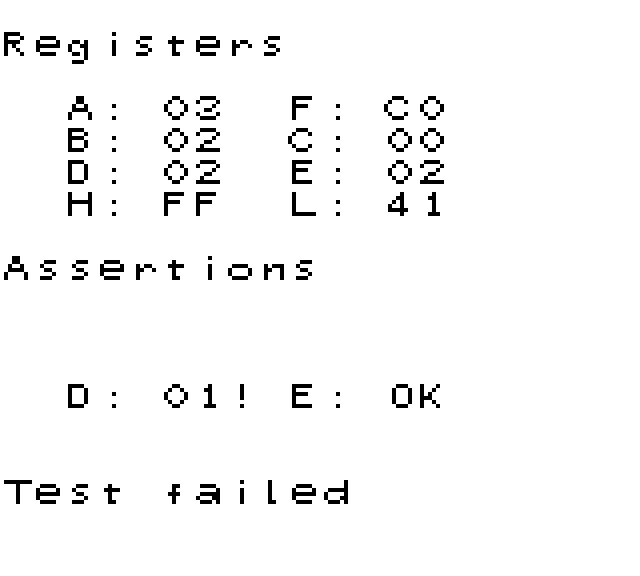
\includegraphics[width=5cm]{images/failed-ppu-timing-test}\\
    \caption{Output of PPU timing test \texttt{ppu\_intr\_2\_mode3\_timing}}
    \label{fig:failed-ppu-timing-test}
\end{figure}

The timer and \glspl{mbc} have great accuracy, and don't have any problems as far as the tests can tell. This is important, in particular for the timer, because multiple timing tests rely on the timer functioning. As such, having this part of the emulator work reliable is vital to ensuring the other tests work properly.

Finally, the \gls{apu} performs very poorly. This is firstly due to the complexity of the different channels - they all have several mechanisms working separately, and if only one of them behaves wrongly then the whole set of tests will fail. Furthermore, the majority of these tests come from the SameSuite\ftnt{https://github.com/LIJI32/SameSuite} test suite. These tests differ from other because they use the \texttt{PCM12} and \texttt{PCM34} registers of the \gls{gbc}, to directly inspect the output of each channel \cite[Audio Details]{pandoc}. These allows the tests to check with much more precision that the emulator works, making the test significantly more stringent. Although this is an obvious indicator that the \gls{apu} needs to be reworked and fixed, this doesn't impact the user experience, or at least not that of a casual user, as the audio of the game doesn't sound off when being used.

Seeing the total of tests passed is also of interest. The total success rate is 52.8\%, but is value is strongly influenced by the fact almost half of the tests are for the fauly \gls{apu} (82 tests out of 191). If these tests are filtered out, we get a total of 109 tests, of which 96 pass, giving a success rate of 88\%. A really good result, given the emulator was written in a short period of time with no prior experience.

\section{Relative Accuracy}

After verifying the accuracy of the emulator by itself, using automated tests, we may also want to compare it to other existing \gls{gb} emulators, and see how it does in contrast with them.

Thankfully, a tool for this already exists: ``GBEmulatorShootout''\ftnt{https://github.com/daid/GBEmulatorShootout}. It automatically tests \gls{gb} emulators, and displays their results in a large table, allowing for the comparison of emulators' accuracy. 

The way the tool works is that each emulator it supports must have a matching file, to allow downloading the emulator's executable and running it with a given test \gls{rom}. The program then regularly screenshots the emulator's window, and compares it with the expected visual output of the test. This means the tool expects the emulator's window to only contain the graphical output of the emulator.

This means that adding this emulator to the tool required changes to the tool's source code. Indeed, this emulator has two notable distinctions to other emulators tested by the tool. First and foremost, this emulator is not based on an executable - it is instead \textit{browser based}, meaning that simply running the emulator's file is not possible. The second difference is that the emulator's output doesn't cover the whole window, as there is an additional UI around it. We must thus instead find a way to extract the emulator's output from the window.

To do this, we will use web development techniques to automate the tests. Selenium\ftnt{https://www.selenium.dev/} is a tool that allows programmatically opening a browser and running actions on it, mimicking those of a user. In this case, these actions would be opening the emulator's website, and uploading the \gls{rom} to the emulator, as a user would do. Because the rest of the tool is written in Python\ftnt{https://www.python.org/}, we will use the \texttt{selenium} Python package\ftnt{https://pypi.org/project/selenium/}. See figure \ref{fig:selenium-testing} for the code to setup the emulator, and the code to run a \gls{rom} on it. Opening the window and accessing the emulator is quite simple (see lines~2--6), as we must just open the window at a given URL. We may note the script also does two additional actions: the first is enabling ``triple speed mode'' (line 5), to make the tests run faster. We also open the ``Settings'' tab of the sidebar (line~6), as this is where the console selection (\gls{dmg} or \gls{gbc}) is done. This is relevant because some tests are designed for a console in particular, and the only way to switch the console on this emulator is via this UI.

\begin{figure}[h]
    \begin{minted}{python}
class Emmy(Emulator):
    def setup(self):
        self.driver = webdriver.Chrome("emu/chromedriver_win32/chromedriver.exe")
        self.driver.get("https://emmy-gbc.vercel.app/")
        self.driver.find_element(value="emu-speed").click()
        self.driver.find_element(value="drawer-section-settings").click()

    def startProcess(self, rom, *, model, required_features):
        model_btn_id = {DMG: "dmg-mode", CGB: "cgb-mode"}.get(model)
        if model_btn_id is None: # console not supported
            return None
        self.driver.find_element(value=model_btn_id).click()
        rom_path = os.path.abspath(rom)
        self.driver.find_element(value="rom-input").send_keys(rom_path)
        try: # if an alert appeared, it means the rom is incompatible
            self.driver.switch_to.alert.accept()
            return None
        except: # no alert, so error thrown, so the rom is compatible
            return self.driver
    \end{minted}
    \caption{Setup and run code to automate emulator testing}
    \label{fig:selenium-testing}
\end{figure}

Once the emulator is setup, the test \gls{rom} must be handled. First, the desired console model is checked, and the appropriate console is selected in the UI (lines~9--12). This is done my matching the model ID to the ID of the button that selects said console, and clicking the button with that ID. The test \gls{rom} may then be uploaded, by pressing the ``Import a ROM'' button, and entering the \gls{rom}'s path. We must also check if an alert is raised in the browser (lines~15--19) - this occurs if an error occurs when reading a \gls{rom}, usually because the \gls{mbc} is not supported.

The second part of automated testing requires monitoring the emulator, and verifying if the test succeeded or failed. GBEmulatorShootout requires taking screenshots of the emulator frequently, and comparing the screenshot to an image of the expected result. This method implies storing an additional image for each test \gls{rom}, but comes with the advantage that no complex code is required to look into the emulator's state for other indicators of success (like what was done in this project's frontend, see subsection \ref{sec:testing-ui}).

To do this, we must extract the image from the \texttt{<canvas/>} element the emulator's frontend draws in, and convert it to an appropriate Python object (see figure \ref{fig:selenium-screenshot}). We first fetch the output canvas by it's ID, and execute a small JavaScript function to retrieve the image inside the canvas, in a PNG format. This data is then decoded, and used to create an image, that is resized to the correct size (as the emulator's screen may be upscaled by the browser).

\begin{figure}[h]
    \begin{minted}{python}
def getScreenshot(self):
    canvas = self.driver.find_element(value="emulator-frame")
    canvas_base64 = self.driver.execute_script(
    	"return arguments[0].toDataURL('image/png').substring(21);", 
    	canvas
    )
    canvas_png = base64.b64decode(canvas_base64)
    large_image = PIL.Image.open(io.BytesIO(canvas_png))
    small_image = large_image.resize((160, 144), PIL.Image.NEAREST)
    return small_image
    \end{minted}
    \caption{Code to get the emulator's output with Selenium}
    \label{fig:selenium-screenshot}
\end{figure}

After other minor tweaks to GBEmulatorShootout's code to support web-based emulators, the test script can be run to compile the results and be able to finale compare our emulator to others. The results are accessible online at \url{https://n1ark.github.io/GBEmulatorShootout/} (see~figure \ref{fig:gb-shootout}). The website to access the results is made of a large table, with on the X axis the emulator running the test \gls{rom}, and on the Y axis the name of the test \gls{rom}. Emulators are ordered from most accurate (most tests passed) to least accurate, from left to right. The tool currently supports 239 test \glspl{rom}, for 14 emulators.

\begin{figure}[h]
    \centering
    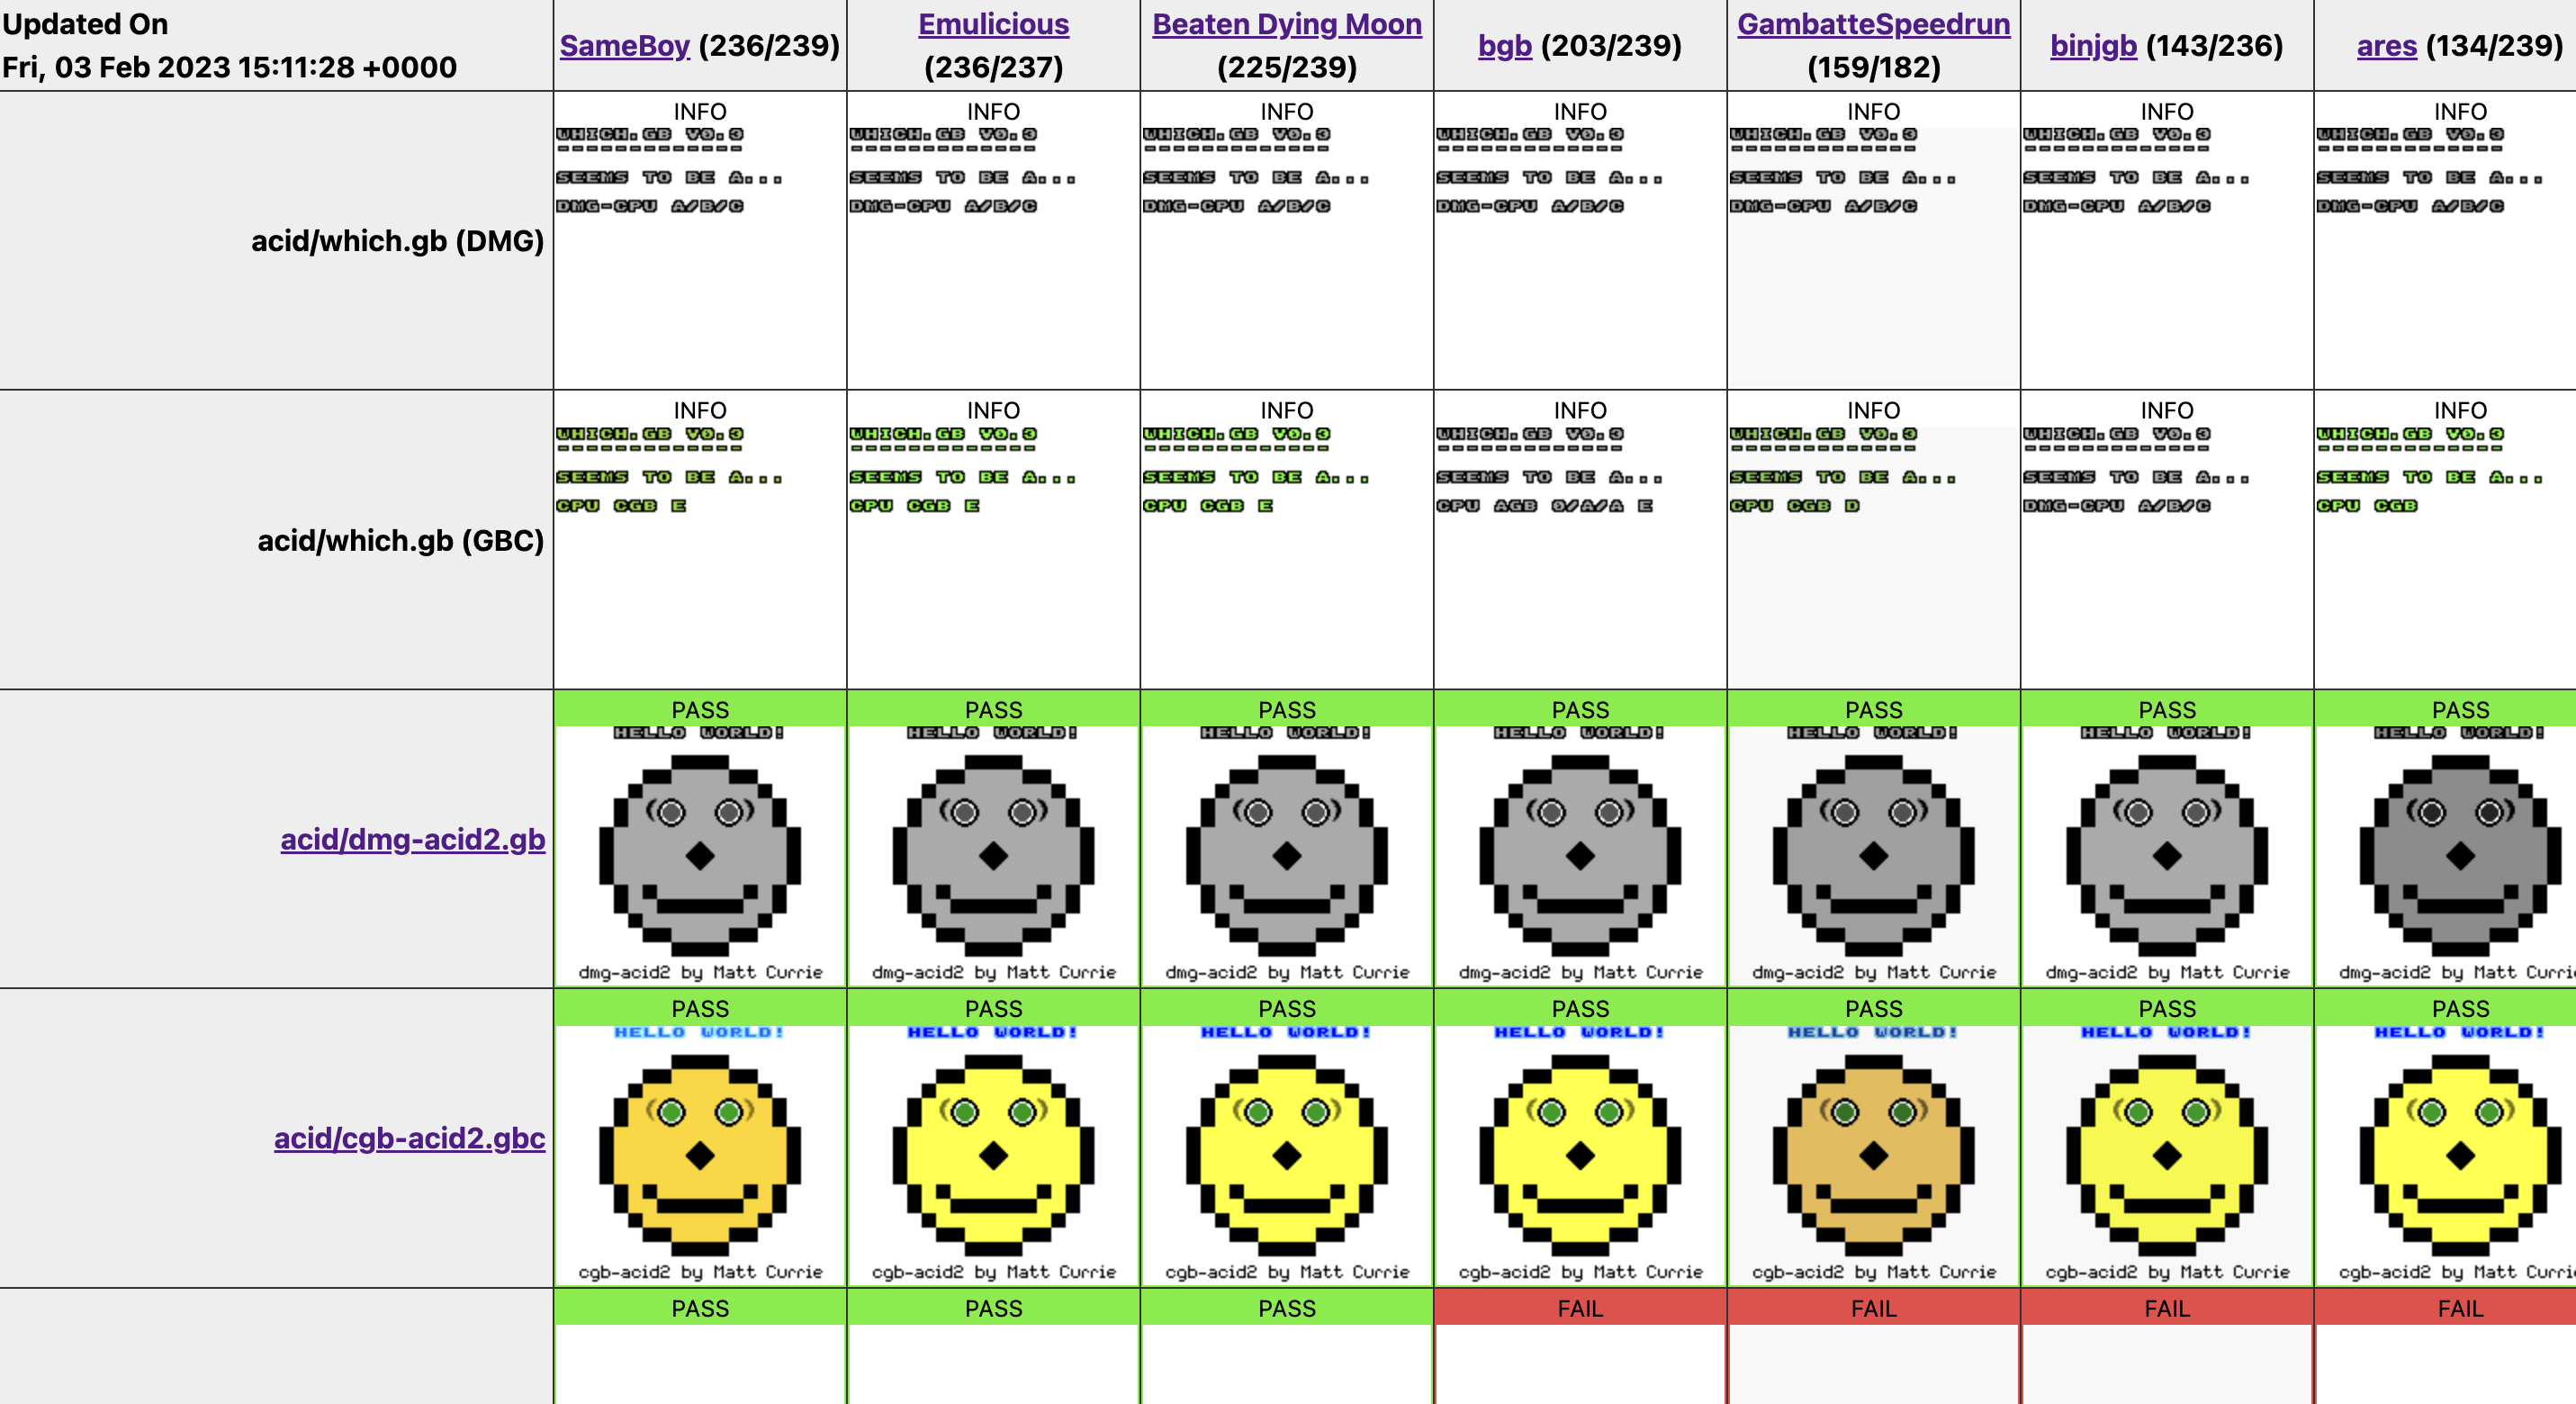
\includegraphics[width=15cm]{images/gb-shootout}\\
    \caption{Screenshot of the UI of \texttt{GBEmulatorShootout}}
    \label{fig:gb-shootout}
\end{figure}

We may first notice that the present emulator passes 118 out of 236 tests (3 tests are skipped because the emulator doesn't support the ``Super Game Boy''), ranking it 9th of the 14 tested emulators. It is relevant here to note that most of these other emulators have existed for several years now, and have been worked on by many people.

We may also want to use this table to compare the performance of this emulator to others, by looking at its success rate for tests of different components compared to others (see figure \ref{fig:stats-tests-relative}). Note that if an emulator cannot run a test (because it doesn't support a feature needed by the test), the test is skipped, rather than counted as failed. This explains why \mbox{``VisualBoyAdvance-M''} has a success rate of 57.1\% but is ranked lower than Emmy.

\begin{figure}[h]
    \centering
    \begin{tabular}{|l|l|l|l|l|l|l|l|}
    \hline
    \textbf{Emulator} & \textbf{Tests Run} & \textbf{CPU} & \textbf{PPU} & \textbf{Timer} & \textbf{MBCs} & \textbf{APU} & \textbf{All} \\ \hline
	
	\textbf{SameBoy} & 239 & 100.0\% & 91.9\% & 100.0\% & 100.0\% & 100.0\% & 98.7\% \\
	\textbf{Emulicious} & 237 & 98.5\% & 100.0\% & 100.0\% & 100.0\% & 100.0\% & 99.6\% \\
	\textbf{Beaten Dying Moon} & 239 & 100.0\% & 97.3\% & 100.0\% & 97.1\% & 85.9\% & 94.1\% \\
	\textbf{bgb} & 239 & 74.6\% & 91.9\% & 100.0\% & 97.1\% & 82.4\% & 84.9\% \\
	\textbf{GambatteSpeedrun} & 182 & 98.5\% & 81.1\% & 100.0\% & 57.1\% & 100.0\% & 87.4\% \\
	\textbf{binjgb} & 236 & 84.6\% & 63.9\% & 92.3\% & 74.3\% & 29.4\% & 60.6\% \\
	\textbf{ares} & 239 & 82.1\% & 51.4\% & 38.5\% & 80.0\% & 29.4\% & 56.1\% \\
	\textbf{mGBA} & 233 & 83.1\% & 52.8\% & 92.3\% & 90.6\% & 20.0\% & 57.1\% \\
	
	\hline	
	\textbf{Emmy} & 236 & 76.9\% & 45.9\% & 100.0\% & 79.4\% & 10.6\% & 50.0\% \\
	\hline
	
	\textbf{VisualBoyAdvance-M} & 182 & 53.7\% & 45.9\% & 76.9\% & 62.9\% & 60.7\% & 57.1\% \\
	\textbf{PyBoy} & 143 & 32.1\% & 17.2\% & 38.5\% & 90.6\% & 0.0\% & 40.6\% \\
	\textbf{Goomba} & 232 & 30.8\% & 8.6\% & 7.7\% & 59.4\% & 3.5\% & 20.7\% \\
	\textbf{no\$gmb} & 236 & 35.4\% & 22.2\% & 0.0\% & 20.0\% & 2.4\% & 17.8\% \\
	\textbf{KiGB} & 231 & 29.2\% & 20.0\% & 0.0\% & 12.9\% & 2.4\% & 14.7\% \\\hline
		
    \end{tabular}
    \caption{Success rate of emulators for different components, sorted by total passed tests}
    \label{fig:stats-tests-relative}
\end{figure}

This table is a good indicator of where our emulator, Emmy, performs well and where it doesn't, compared to other \gls{gb} emulators. For instance, it has a really accurate timer, compared to emulators ranked around it. This also emphasizes the fact that its \gls{cpu} is of an accuracy similar to that of the higher accuracy emulators, passing almost 80\% of tests. It also helps see that only very high accuracy emulators manage to pass the \gls{apu} tests. The only outliar seems to be VisualBoyAdvance-M, with an \gls{apu} success rate of 60.7\%. However, when inspecting the test results, we notice that most of the \gls{apu} tests weren't run on it - this is because it doesn't have support for the \texttt{PCM12} and \texttt{PCM34} registers these tests use. If we add the un-run tests to the percentage, we end with 17 tests passed out of 85, or a 20\% success rate, in line with the success rate of similar emulators. This further shows that creating an accurate \gls{apu} is challenging, especially given the standards of the used test \glspl{rom}.

\section{Performance and Usability}

Aside from accuracy, we may want to measure how performant the emulator is, and how usable it is. The former is important, because most emulators offer a ``turbo mode'', allowing the emulator to run the \gls{gb} faster. The latter is important because many emulators tend to be inconvenient, as they are oriented towards experienced user.

To measure performance, the most relevant metric is frame time: the time needed in milliseconds to draw a frame (this, of course, includes the rendering of the frame but also all the processing that goes before). The emulator's frontend already comes with a measure of frame time - as such, we just need to select on what \gls{rom} the test will be performed, and how the measure will be taken.

For the \gls{rom}, the performance will be measured on 4 distinct \glspl{rom}, all outlining different uses of the emulator. These \glspl{rom} are:

\begin{compactitem}
	\item ``The Legend of Zelda: Link's Awakening'', a \gls{dmg} game. It is quite simple and shouldn't be too memory intensive. It will help outline the average performance on the \gls{dmg}.
	\item The \texttt{cpu\_instrs} test \gls{rom}. It's advantage is that it is quite long, and it's purpose is to test the entirety of the \gls{cpu}, meaning it will be very processor-intensive.
	\item ``The Legend of Zelda: Oracle of Ages'', a \gls{gbc} game. It is similar to the previous Zelda \gls{rom}, but was built for the \gls{gbc}, meaning it likely requires more resources to run.
	\item ``Alone in the Dark: The New Nightmare'', a \gls{gbc} game. This is a very complex game released for the \gls{gbc}, that supports ``3D-scenes'', and very regularly changes the color palette registers\cite[Tricky-to-emulate games]{gbdev_wiki}. Both of these properties combined should make this \gls{rom} slower, making it a hypothetical ``upper-bound'' on frame time.
\end{compactitem}

As for how to measure the frame time, the frame time of every frame will be summed and average, over the first 10 million cycles, to give a more accurate measure. See figure \ref{fig:frame-time-results} for the results.

From this table we can notice two things. First, it is that \gls{dmg} games run faster than \gls{gbc} games. This can be due to the double speed mode, that forces the emulator to run twice as many instructions, or to the fact that the \gls{ppu} logic with colour is more complex and needs to be optimised. Secondly we may look at the average frame times of these \glspl{rom}. 

The \gls{gb} runs at 60 frames per second, meaning a frame must last at most $\frac{1}{60}=16.6\text{ms}$. We may calculate the maximum speed increase attainable for a frame time via the formula~$\frac{1000}{\text{frame time} * 60}$, or $(\frac{1000}{\text{frame time} * 60}-1)*100$ to get an increase percentage. For instance, for ``The Legend of Zelda: Link's Awakening'', the maximum speed increase could be of around 279\%.

\begin{figure}[h]
    \centering
    \begin{tabular}{|l|l|l|l|}
    \hline
    \textbf{Console} & \textbf{ROM} & \textbf{Frame time} (ms) & \textbf{Speed increase} \\ \hline

	\multirow{2}{*}{\textbf{\gls{dmg}}} 
	& The Legend of Zelda: Link's Awakening & 4.39 & 279\% \\\cline{2-4}
	& \texttt{cpu\_instrs} & 5.43 & 207\% \\\hline
	\multirow{2}{*}{\textbf{\gls{gbc}}} 
	& The Legend of Zelda: Oracle of Ages & 4.89 & 241\% \\\cline{2-4}
	& Alone in the Dark: The New Nightmare & 5.78 & 188\% \\\hline
	
    \end{tabular}
    \caption{Average frame time of different \glspl{rom}}
    \label{fig:frame-time-results}
\end{figure}

This is a satisfiable value - a speed increase of 200\% is good enough for most uses. Many emulators provide speed increases much superior to this, however this is because these emulators are often written in compiled languages like C++ or Rust, and will thus run much faster than an interpreted language like JavaScript.

WebAssembly\ftnt{https://webassembly.org/} is a low-level language made for browsers, ressembling assembly language. It is designed for efficiency, and would thus be a great pick for a browser-based emulator as it runs faster~\cite{wasm-faster}. Languages like C, C++ and Rust can be compiled to WebAssembly via tools like emscripten\ftnt{https://emscripten.org/}, allowing for great performance with portable code. Examples of such emulators playable from the browser include GBEmu\ftnt{https://github.com/BlueBlazin/gbemu}, an emulator written in Rust that is compiled to WebAssembly and that can thus be played from a browser.


This would however require a full rewrite of the code, since TypeScript and C++ have little in common in terms of syntax. Another simpler alternative to convert the emulator's code to a WebAssembly-compilable language is using AssemblyScript\ftnt{https://www.assemblyscript.org/}, a language similar to TypeScript.

Research has been done to convert the project's code to AssemblyScript, and the progress so far can be seen on the \texttt{assembly-script} branch\ftnt{https://github.com/N1ark/gbc-emulator/tree/assembly-script}. However, because AssemblyScript targets such a low-level language, many TypeScript constructs are not (yet) available in it, such as arrow functions, or dynamic objects. Although the implemented emulator doesn't use these features extensively and most components were succesfully migrated to AssemblyScript, the \gls{cpu} uses arrow functions for all instructions - a succesful conversion of the entire emulator would thus require a lengthy rewrite of the \gls{cpu}. This project was thus abandoned in favour of additional features in the emulator's core and frontend. An example of \gls{gb} emulator in AssemblyScript is wasmboy\ftnt{https://github.com/torch2424/wasmboy/}.

In terms of usability, the presented emulator fullfils most of the specification, with some specifications of lower importance having been left out. These include:

\begin{compactitem}
	\item The user cannot, currently, download the save of their game (code U4).	 The save file is instead stored in the browser. Some research was done to allow saving the emulator's state to the BESS\ftnt{https://github.com/LIJI32/SameBoy/blob/master/BESS.md} save format, however this required a lot more effort so priority was shifted on other features, as the existing save system was deemed sufficient.
	\item The emulator's frontend does not provide a way to add breakpoints to the emulation (code U7). This feature was initially supported from the browser's console, but it's implementation wasn't satisfactory. A possible improvement to the emulator would thus be support for such breakpoints, maybe in a format similar to that of the current ``Watch Expressions'' menu.
	\item The implemented emulator cannot currently be downloaded as a local app (code N3). This could however be added quite easily, using a tool like Electron\ftnt{https://www.electronjs.org/} that allows converting web applications to desktop apps. Another option is converting the web-app into a Progressive Web App (PWA)\ftnt{https://web.dev/progressive-web-apps/}, allowing users to ``download'' the web-app and use it while offline.
\end{compactitem}

All of these specifications are however of low importance, and are mainly small quality of life features. Other possible improvements could include more debugging tools (such as a way to inspect the \gls{apu}'s raw output), or more features added to the emulator's core, like support for other \glspl{mbc} (like the MBC6, MBC7, or MMM01 \cite[MBCs]{pandoc}), the real time clock of the MBC3, additional outputs of the \gls{gb} like the Game Boy Printer or the Game Boy Camera \cite{pandoc}, and support for the Link Cable, allowing multiple Gameboys to play together \cite[Serial Data Transfer]{pandoc}.

\chapter{Legal, Social, Ethical and Professional Issues}

\section{Privacy}

This piece of software is safe to use in terms of privacy - it runs entirely locally, with no data ever being sent from the user to the server. There are no cookies, and the only forms of storage used are localStorage\ftnt{https://developer.mozilla.org/en-US/docs/Web/API/Window/localStorage} and localForage\ftnt{https://github.com/localForage/localForage}, both of which are local and offline. 

localStorage is handled by the browser, so it is the user's responsability to ensure that they use a secure browser. 

localForage is an open source library, allowing for more transparence - one could go through the source code to verify that it is safe as well. Whenever a new update is released, we may simply verify that the modified code is still safe, and then configure the project to use the new version in the \texttt{package.json} file.

\section{Legality}

The \glsdesc{gb} is a copyrighted console, owned by Nintendo, but making an emulator for it is deemed legal as long as it is done following a ``clean room'' design \cite{emulation_white_paper}. This was ruled via a series of court appeals between console manufacturers and groups that produce emulators, with the latter consistently winning the appeal. This was the case for Sony Computer Entertainment America v. Connectix Corporation trial, that deemed that the ``Virtual Game Station'' PlayStation emulator wasn't a copyright infringement on Sony, and that Connectix's reverse engineering of the original PlayStation's BIOS was fair use \cite{sony_v_connectix}. This project was developed using online resources about the \gls{gb} compiled by people who reverse engineered the \gls{gb}, and as such was developed with a clean room design too.

Although distributing the emulator is legal, distributing the BIOS (Basic Input/Output System) of the console with the emulator is not, as it is still copyrighted software \cite{emulation_white_paper}. Because acquiring such BIOS is however not illegal as long as the user owns the console, a user is free to use their own BIOS in the emulator (see sub section \ref{sec:settings-ui}). The emulator otherwise simulates the effect of the BIOS on the system, by setting up all the necessary memory and registers.

Distributing copyrighted game \glspl{rom} is also not allowed - this is why the user must upload the \gls{rom} they want to use themselves. The software does not upload the \gls{rom}, and simply stores it in local storage.

\section{Integrity}

This piece of software was developed with integrity, always thinking critically on what was developed, and with no intention to harm others. This report has also been written with honesty, without attempting to withhold information on the resulting software. No acquired data was falsified or modified to fit a narrative.

The produced software is also open source, and available at \url{https://github.com/N1ark/gbc-emulator}. This means it can be used by others to create similar emulators, or for educational purposes. Other users may also contribute to the project, or fix issues it has.

Overall, this software was developed with the British Computer Society's Code of Conduct \& Code of Good Practice\ftnt{https://www.bcs.org/media/2211/bcs-code-of-conduct.pdf} in mind, and all of its relevant rules were followed.

\chapter{Conclusion and Future Work}

\section{Conclusion}

This project helped outline the typical structure of a an emulator, and in particular that of a \glsdesc{gb} emulator. It describes how the console works in detail, what components it is made of, and how they interact with eachother. It showcased optimisation methods for emulating different components of an emulator, like the \gls{cpu} or the system bus. The resulting software is a fully playable \glsdesc{gb} and \glsdesc{gbc} emulator, that has multiple quality of life features to make the experience more pleasant while also providing debugging tools for retro game and emulator developers. This emulator can be played on both computer and mobile devices, and is of good accuracy compared to other existing emulators.

\section{Future Work}

As it stands the emulator has three main properties that could be improved, each independently one of the other.

The first is improving the accuracy of the emulator. As seen in the evaluation of the project, itd \gls{apu} should be reworked. It is currently lackluster, and represents a part of the system that could be improved without requiring a full re-write, as it is self contained. Other small improvements could be done to improve the accuracy of other components like the \glspl{mbc} or the \gls{ppu}, or to add currently unsupported \glspl{mbc} and accessories. All of these improvements can be done separately and in small increments, and don't entail any breaking changes outside of the emulator's core.

A second important point to be improved in the emulator is its performance. As seen in its evaluation, an average maximum of a 200\% speed increase is reachable. To improve the performance of the emulator (which will be needed if more features are to be added), its performance must be improved substantially. Although code optimisations and caching could improve some of the performance issues, a significant bottleneck is the language used itself. If the emulator were to be entirely rewritten using a language such as AssemblyScript, it would likely run much faster. This would be much more time-consuming of a change, and would requiring updating the front-end to work properly with it, but could yield great performance improvements if done properly.

Finally, the third point to improve on this project is it's frontend. Although it has a good range of available features, it could still be improved to be up to par with other technical emulators. More and better debugging tools could be provided to the user, as well as more customisation options, such as new screen filters, a full-sreen mode or support for input macros.

\clearpage

\printnoidxglossary[type=\acronymtype]

\printnoidxglossary[type=main]

\printbibliography


\end{document}
